% \documentclass[a4paper, technote, compsoc]{IEEEtran}
\documentclass[../../thesis.tex]{subfiles}

\newcommand{\inner}[2]{\left<#1, #2\right>}
\newcommand{\alemap}{\ensuremath{\mathcal{A}}}
\newcommand{\dt}{\ensuremath{\Delta t}}
\newcommand{\pexp}{\ensuremath{\frac{2\gamma}{\left(\gamma-1\right)}}}
\newcommand{\aleX}{\ensuremath{\mathcal{X}}}
\newcommand{\Ah}[1]{\ensuremath{\vb{#1}^{n+1}_h}}
\newcommand{\Ahn}[1]{\ensuremath{\vb{#1}^{n}_h}}


\begin{document}

\section{FOM Calibration}
\label{sec:fom_calibration}
This section is devoted to present the Full Order Model in action.
Certain parameters need to tweaked and defined,
along with consistency checks to validate the simulation.

In Section~\ref{sec:fom_calibration_artificial_viscosity} we show the effects of artificial viscosity,
in Section~\ref{sec:fom_calibration_bdf_convergence_rates} we explore the differences 
between BDF-1 and BDF-2 time integration schemes;
and finally in Section~\ref{sec:fom_calibration_system_forcing} we show how
certain combinations within the parameter space produce unfeasible solutions\footnote{
    Due to the lack of a proper stabilization scheme. 
    We are comfortable with this choice since it was not mandatory to
    showcase our reduction tools.
}, 
and so we explain how to sample within the feasible range.

\subsection{Artificial Viscosity}
\label{sec:fom_calibration_artificial_viscosity}
As stated previously in the document, 
we included an artificial viscosity term in the final formulation
to go around the need for more involved stabilization schemes, such as SUPG\footnote{
Note that we could have used the same hyperreduction scheme,
since the approach is purely algebraic.} 
methods or others alike.

A value needs to be choosen for the viscosity constant~$\varepsilon$.
Initially, it was set to be the square of the mesh size, 
\begin{equation*}
    \varepsilon \sim (\Delta x)^2 \sim 10^{-6}.
\end{equation*}
However, a parametric sweep for different viscosity values showed that
this value, 
no matter how small, was introducing measurable damping into the system.

The actual value that seems correct, keeping the system stable whilst purely convective (at least for the time-scale for which we are solving) seems to be a much smaller one,
\begin{equation*}
    \varepsilon \sim 10^{-10}.
\end{equation*}
In Figure~\ref{fig:artificial_viscosity_comparison} we present a comparison for these two viscosity values.
We show the motion of the fluid at the outflow and a phase plot, to ease the analysis of the correlation between the weak shock wave at the outflow and the piston motion.
The smallest viscosity value, $(10^{-10})$ leads to a convection-like phase plot:
the shape of the input is distorted but the maximum and mimimum values are honored, 
the same path is repeated over and over.
Instead, the solution with a higher viscosity value (or at least the one that we thought would do the job) shows a diffusive pattern, reducing the extrema and changing its path on every pass.
\begin{figure}[!h]
    \centering
    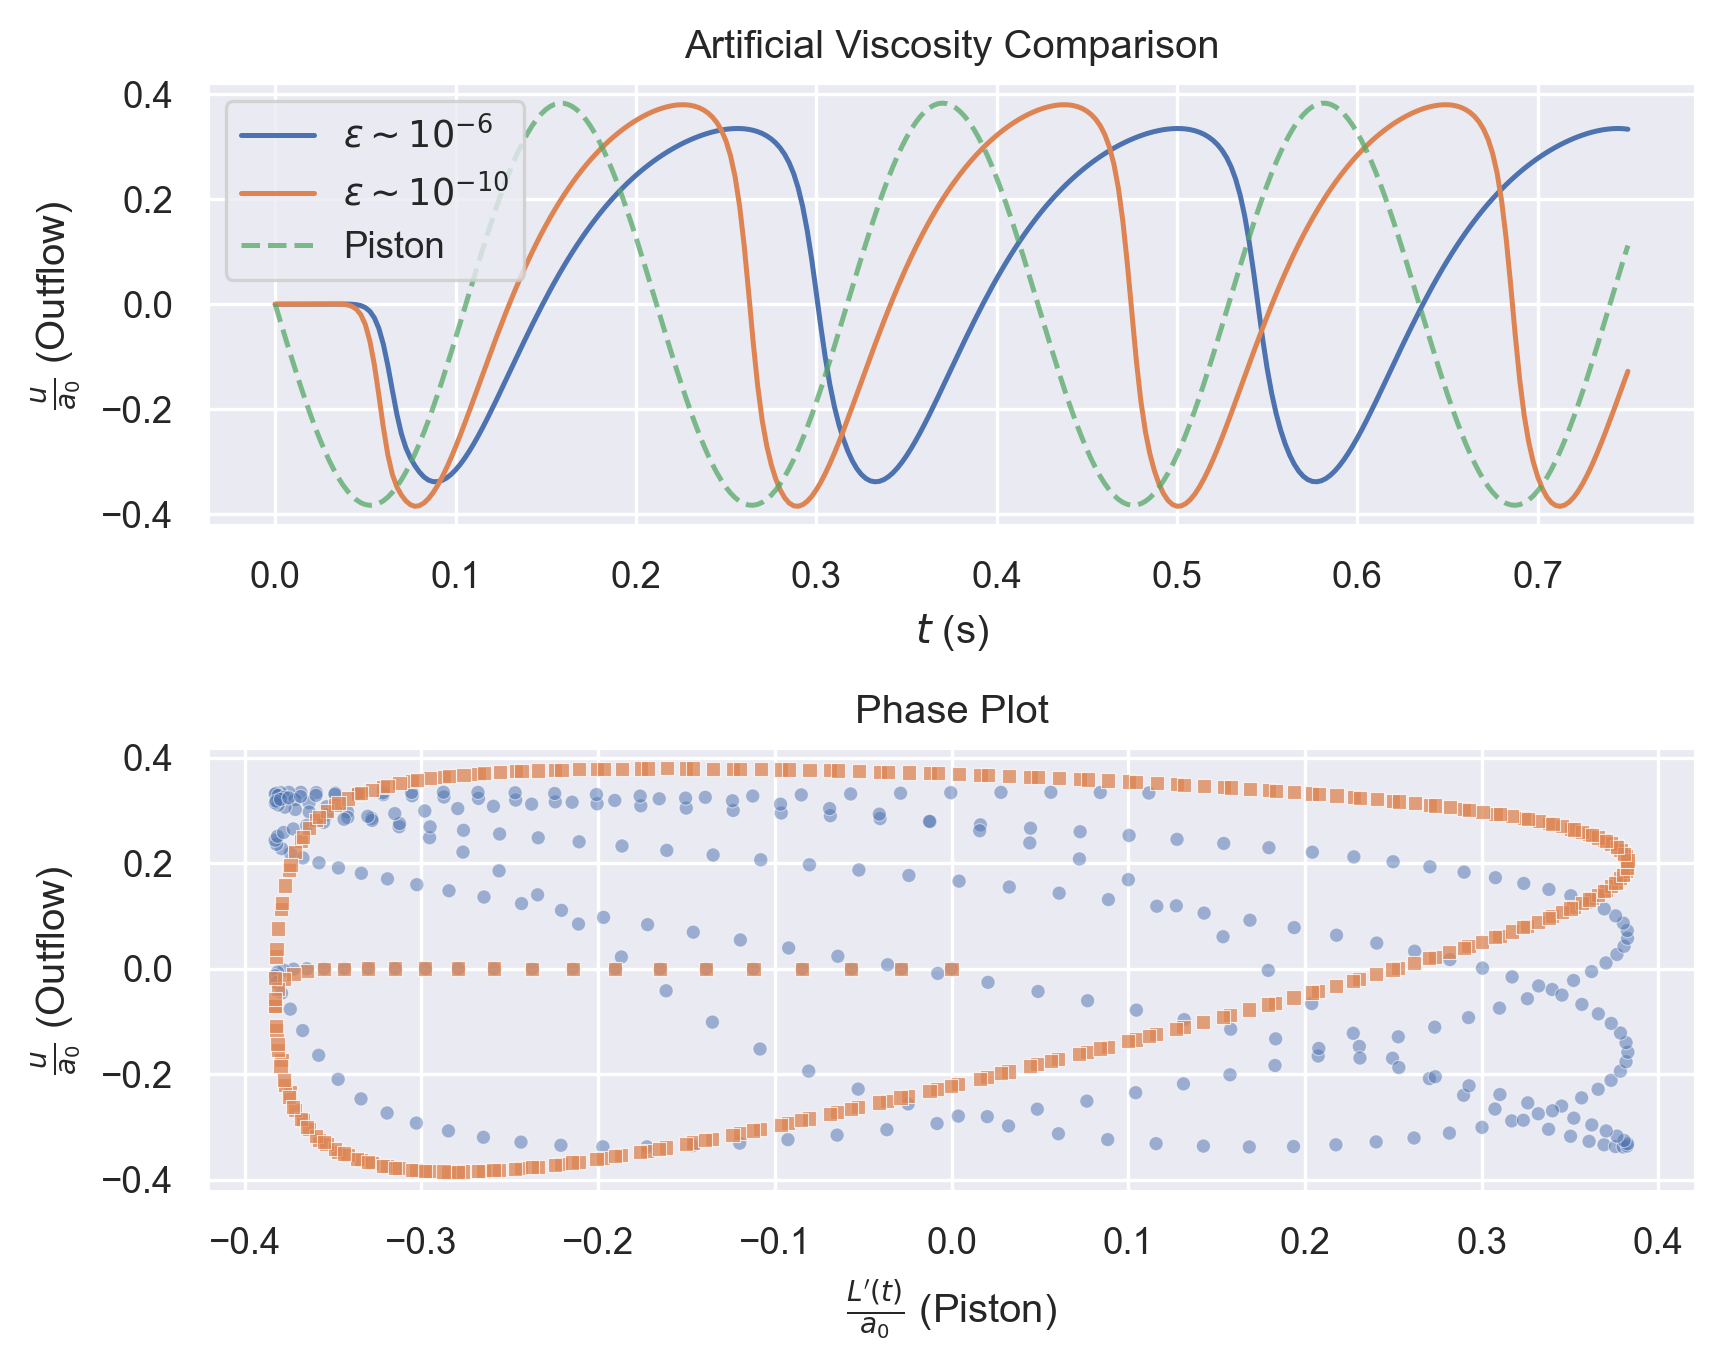
\includegraphics[width=1.0\columnwidth]{research_project/piston/figures/artificial_viscosity/artificial_viscosity_comparison.png}
    \caption{Artificial viscosity comparison.
    (Top) Outer boundary velocities for two different values of the viscosity term.
    In dashed, the piston motion, to help in the visualization of the nonlinear distortion.
    (Bottom) Phase plot between the piston motion (x-axis) and the response at the outer boundary (y-axis) for the same artificial viscosity values.
    Due to the creation of a weak shock wave, the piston motion is distorted.
    However, only the smallest viscosity value ($10^{-10}$) presents a stable phase plot, going over and over the same path. 
    }
    \label{fig:artificial_viscosity_comparison}
\end{figure}
Luckily, the complete reduction scheme\footnote{
    Namely snapshot SVD compression and interpolation coefficients calculation.
}
seems to withstand such a small numerical viscosity term without incurring into round-off errors\footnote{If there were, we could always reduce the plain vanilla Laplace operator $\int \grad u \cdot \grad v \, \text{d}\Omega$ and scale it by $\varepsilon$ right before solving the system.}.

\subsection{BDF Scheme Convergence Rates}
\label{sec:fom_calibration_bdf_convergence_rates}
\mytodo{Convergence rates in space? What would be the expected rate for P1 FE?}
The next concept we are going to look at to check the quality of our simulation is 
the convergence rate for the two time-integration schemes, 
BDF-1 and BDF-2.

We will analyze two convergence plots: the solution itself and mass preservation.
For the solution, since we do not have an analytical reference, we need to establish one numerically.
It will be the one corresponding to the solution for a small timestep, $dt \sim 10^{-4}$.
In Figure~\ref{fig:bdf_convergence_solutions} we present the convergence rates for the solution,
and in Figure~\ref{fig:bdf_convergence_mass} the ones corresponding to the mass defect.

Expectedly, the BDF-2 scheme ($\sim 2$) decreases twice as fast as the BDF-1 scheme ($\sim 1$).
\begin{figure}[h]
    \centering
    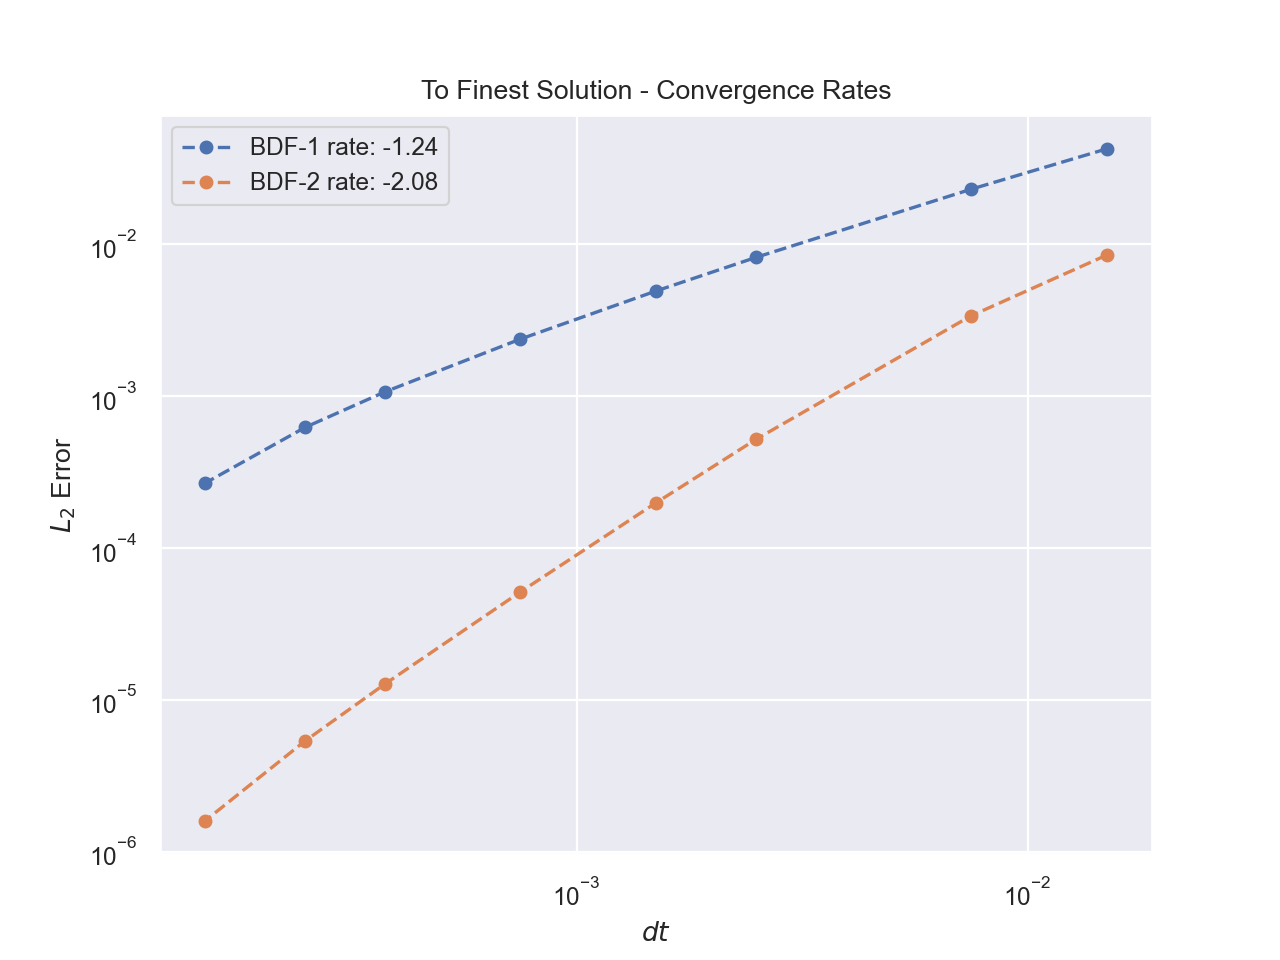
\includegraphics[width=1\columnwidth]{research_project/piston/figures/bdf_convergence/convergence_finest_solution.png}
    \caption{Convergence rates to numerical reference solution.
    Both schemes decrease at the expected rate.}
    \label{fig:bdf_convergence_solutions}
\end{figure}

\begin{figure}[h]
    \centering
    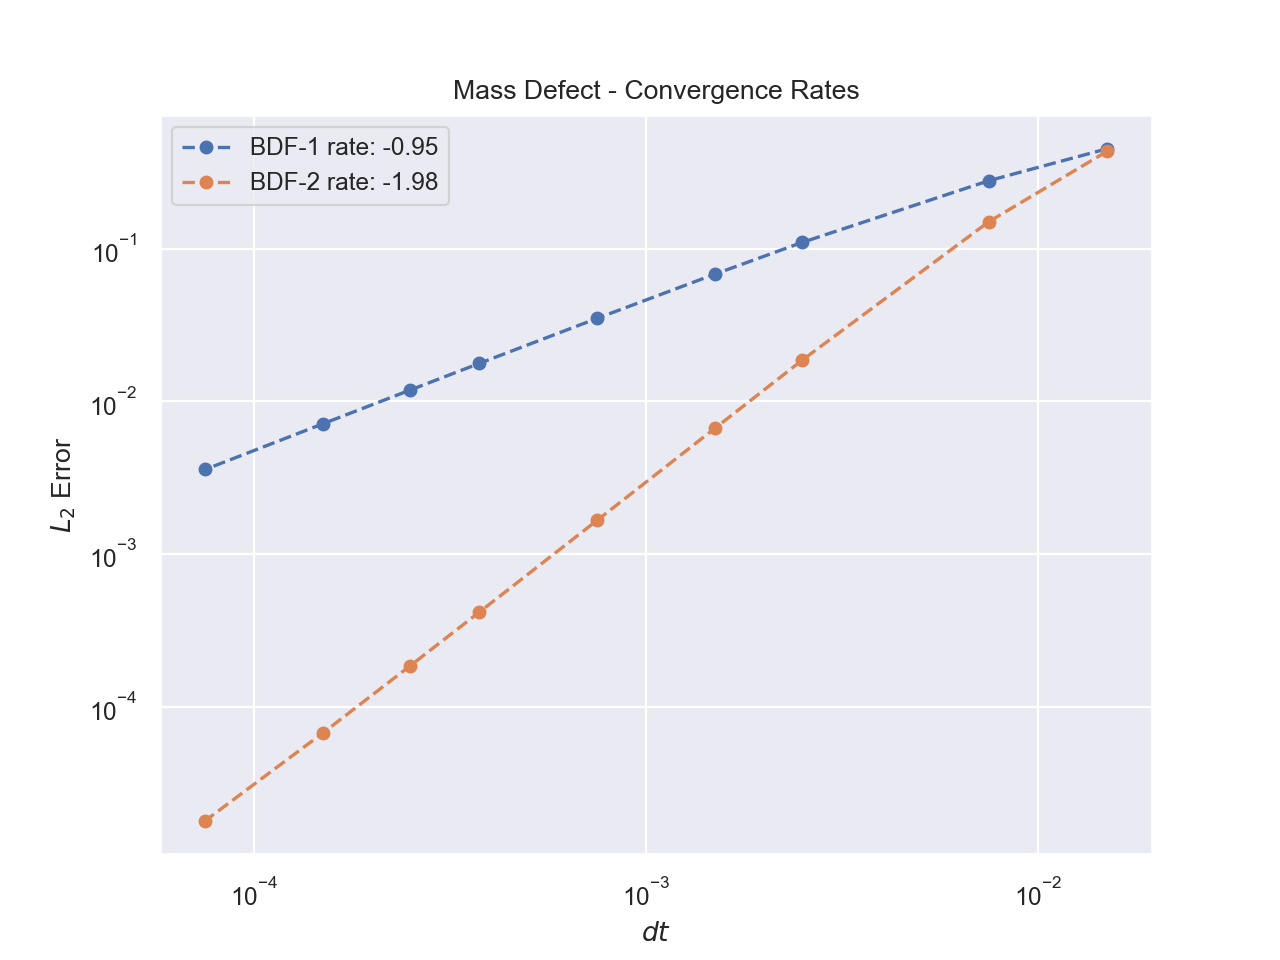
\includegraphics[width=1\columnwidth]{research_project/piston/figures/bdf_convergence/convergence_rates_mass.png}
    \caption{Convergence rates for mass defect.
    Both schemes decrease at the expected rate.}
    \label{fig:bdf_convergence_mass}
\end{figure}

\subsection{Deforming Mesh Effects}

\subsubsection{Mesh Velocity}
\mytodo{Show mass conservation without ALE convective term.}


\subsubsection{Geometric Conservation Law}
As mentioned in the Literature Review regarding deforming meshes, 
in Section \ref{sec:literature_review_deforming_mesh},
a proxy to check to asses how affected is a discretization by a moving mesh
is to attempt the resolution of the constant solution.

This is so because if the discretization is not correctly handling the movement of the mesh,
artificial fluxes of information might be introduced. 
Nevertheless, evidence points towards both directions regarding this test,
succesfully integrating the constant solution seems to be a sufficient but not necessary condition for stability.

Our scheme seems unable to reproduce correctly the constant solution.
This happens in a fixed and moving mesh setting (see Figure~\ref{fig:ale_effect_constant_solution}).
Therefore, we believe it could be due to the accumulation of round-off errors, 
as previous works have reported in the literature \cite{liu2019balancing}.
\begin{figure}[h]
    \centering
    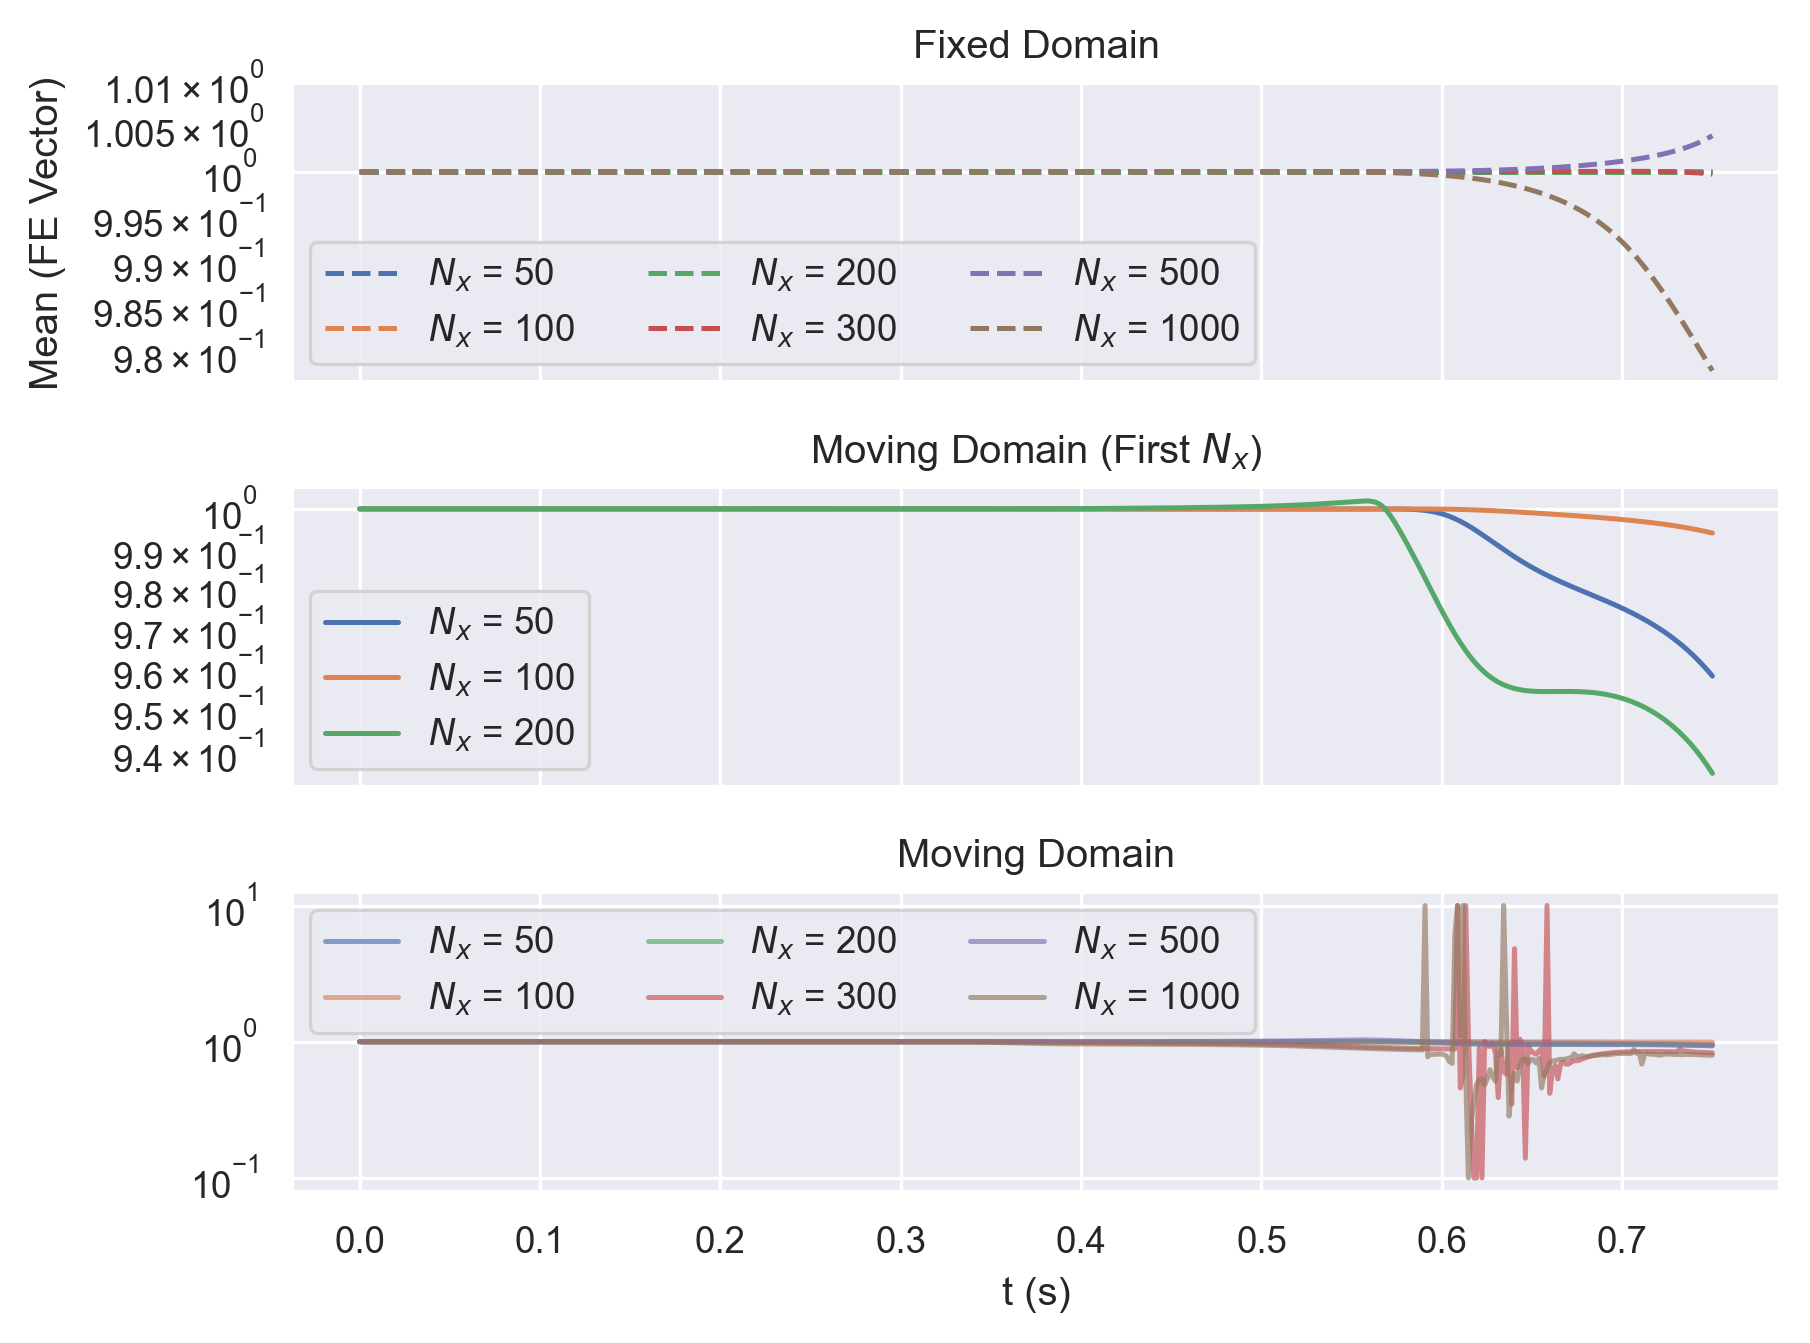
\includegraphics[width=1\columnwidth]{research_project/piston/figures/ale_effect/mean_fe_comparison_constant_solution.png}
    \caption{Constant solution simulation for fixed (top) and moving mesh (middle, bottom).
    The round-off error increases as the number of DoFs increases too ($N_x$). 
    The errors in the fixed mesh take more to accumulate or do not accumulate at all.
    For the moving mesh, for the smallest number of DoFs the solution drifts away from the constant solution.
    In the bottom plot, the values have been clipped to the $[0.01, 10]$ interval.}
    \label{fig:ale_effect_constant_solution}
\end{figure}

In a way, we are surprised that this blowing-up effect does not show up in the piston problem.
We hint towards the fact that, in that context, the constantly changing boundary conditions
somehow lead to balanced round-off errors, which cancel out in time.

Chasing to the detail this behaviour is certainly meaningful, 
but since our reference solution (the piston) does not suffer from these effects,
we limit ourselves to report this behaviour and skip any further investigation, 
as we believe it falls out of the scope of this work. 

\subsection{Parameter Range}
For the construction of the reduced basis we are randomly sampling the parameter space.
We set the range for each parameter in Table~\ref{tab:parameter_range}.

\begin{table}[h]
    \centering
    \caption{Piston parameter range for random sampling.}
    \begin{tabular}{cccc}
    \toprule
        Variable  & Minimum & Maximum & Units 
        \\ \midrule
        $a_0$     & 18      & 25      & m/s \\
        $\omega$  & 15      & 30      & 1/s \\
        $\delta$  & 0.15    & 0.3     & [-]
        \\ \bottomrule
    \end{tabular}
    \label{tab:parameter_range}
\end{table}

% \section{Piston Motion Hyperreduction}

% Piston probes at three different locations.
% It shows that the model contains nonlinearities. 
% \begin{figure}[h]
%     \centering
%     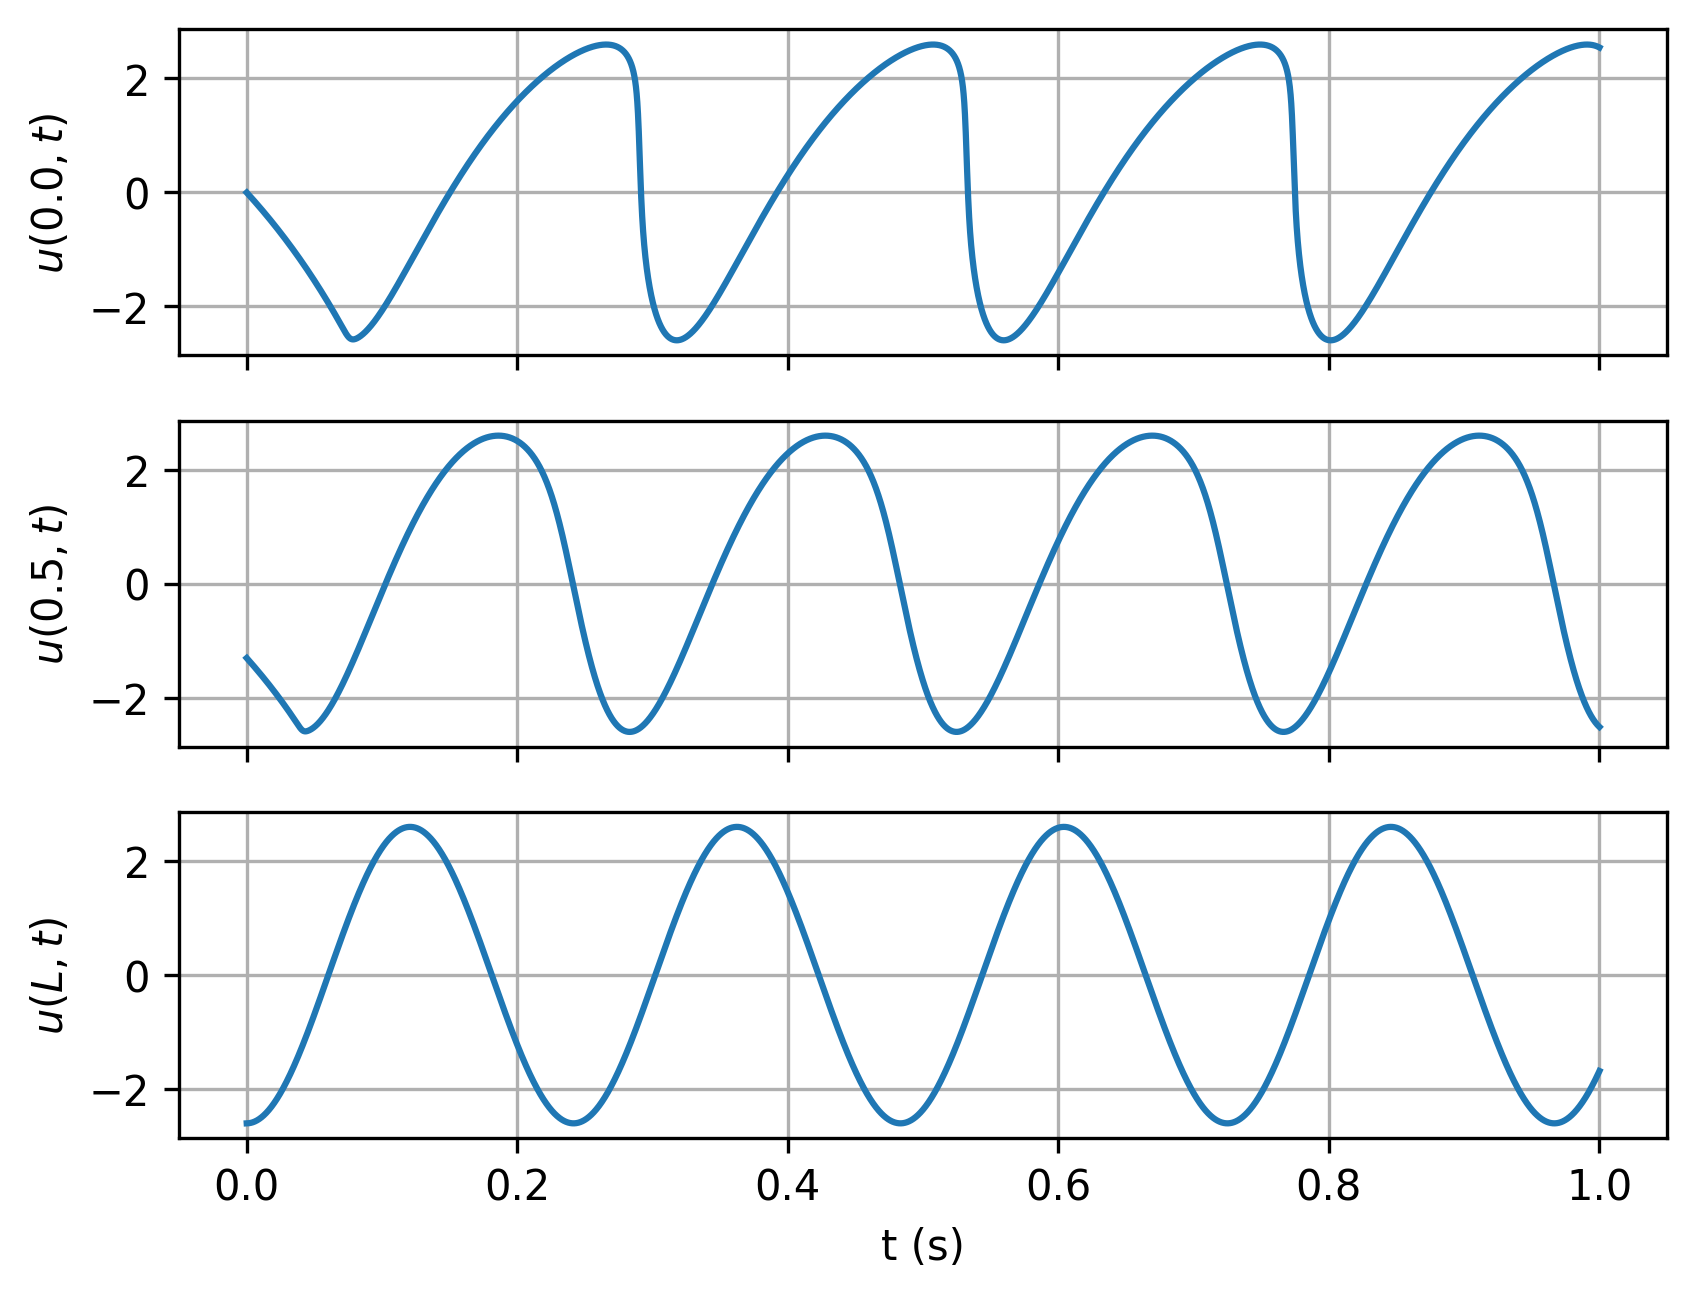
\includegraphics[width=\columnwidth]{research_project/piston/figures/consistency/probes_hifi.png}
%     \caption{Solution probes at three different locations of the piston. 
%     Top: Outflow velocity.
%     Bottom: Piston motion (boundary condition).}
% \end{figure}

% \subsection{Discretization Consistency}
% We use mass conservation as a criteria to determine whether the numerical scheme is consistent.
% Figure~\ref{fig:comparison_bdf} shows plots for mass conservation for the BDF-1 and BDF-2 schemes.

% \begin{figure}[h]
%     \centering
%     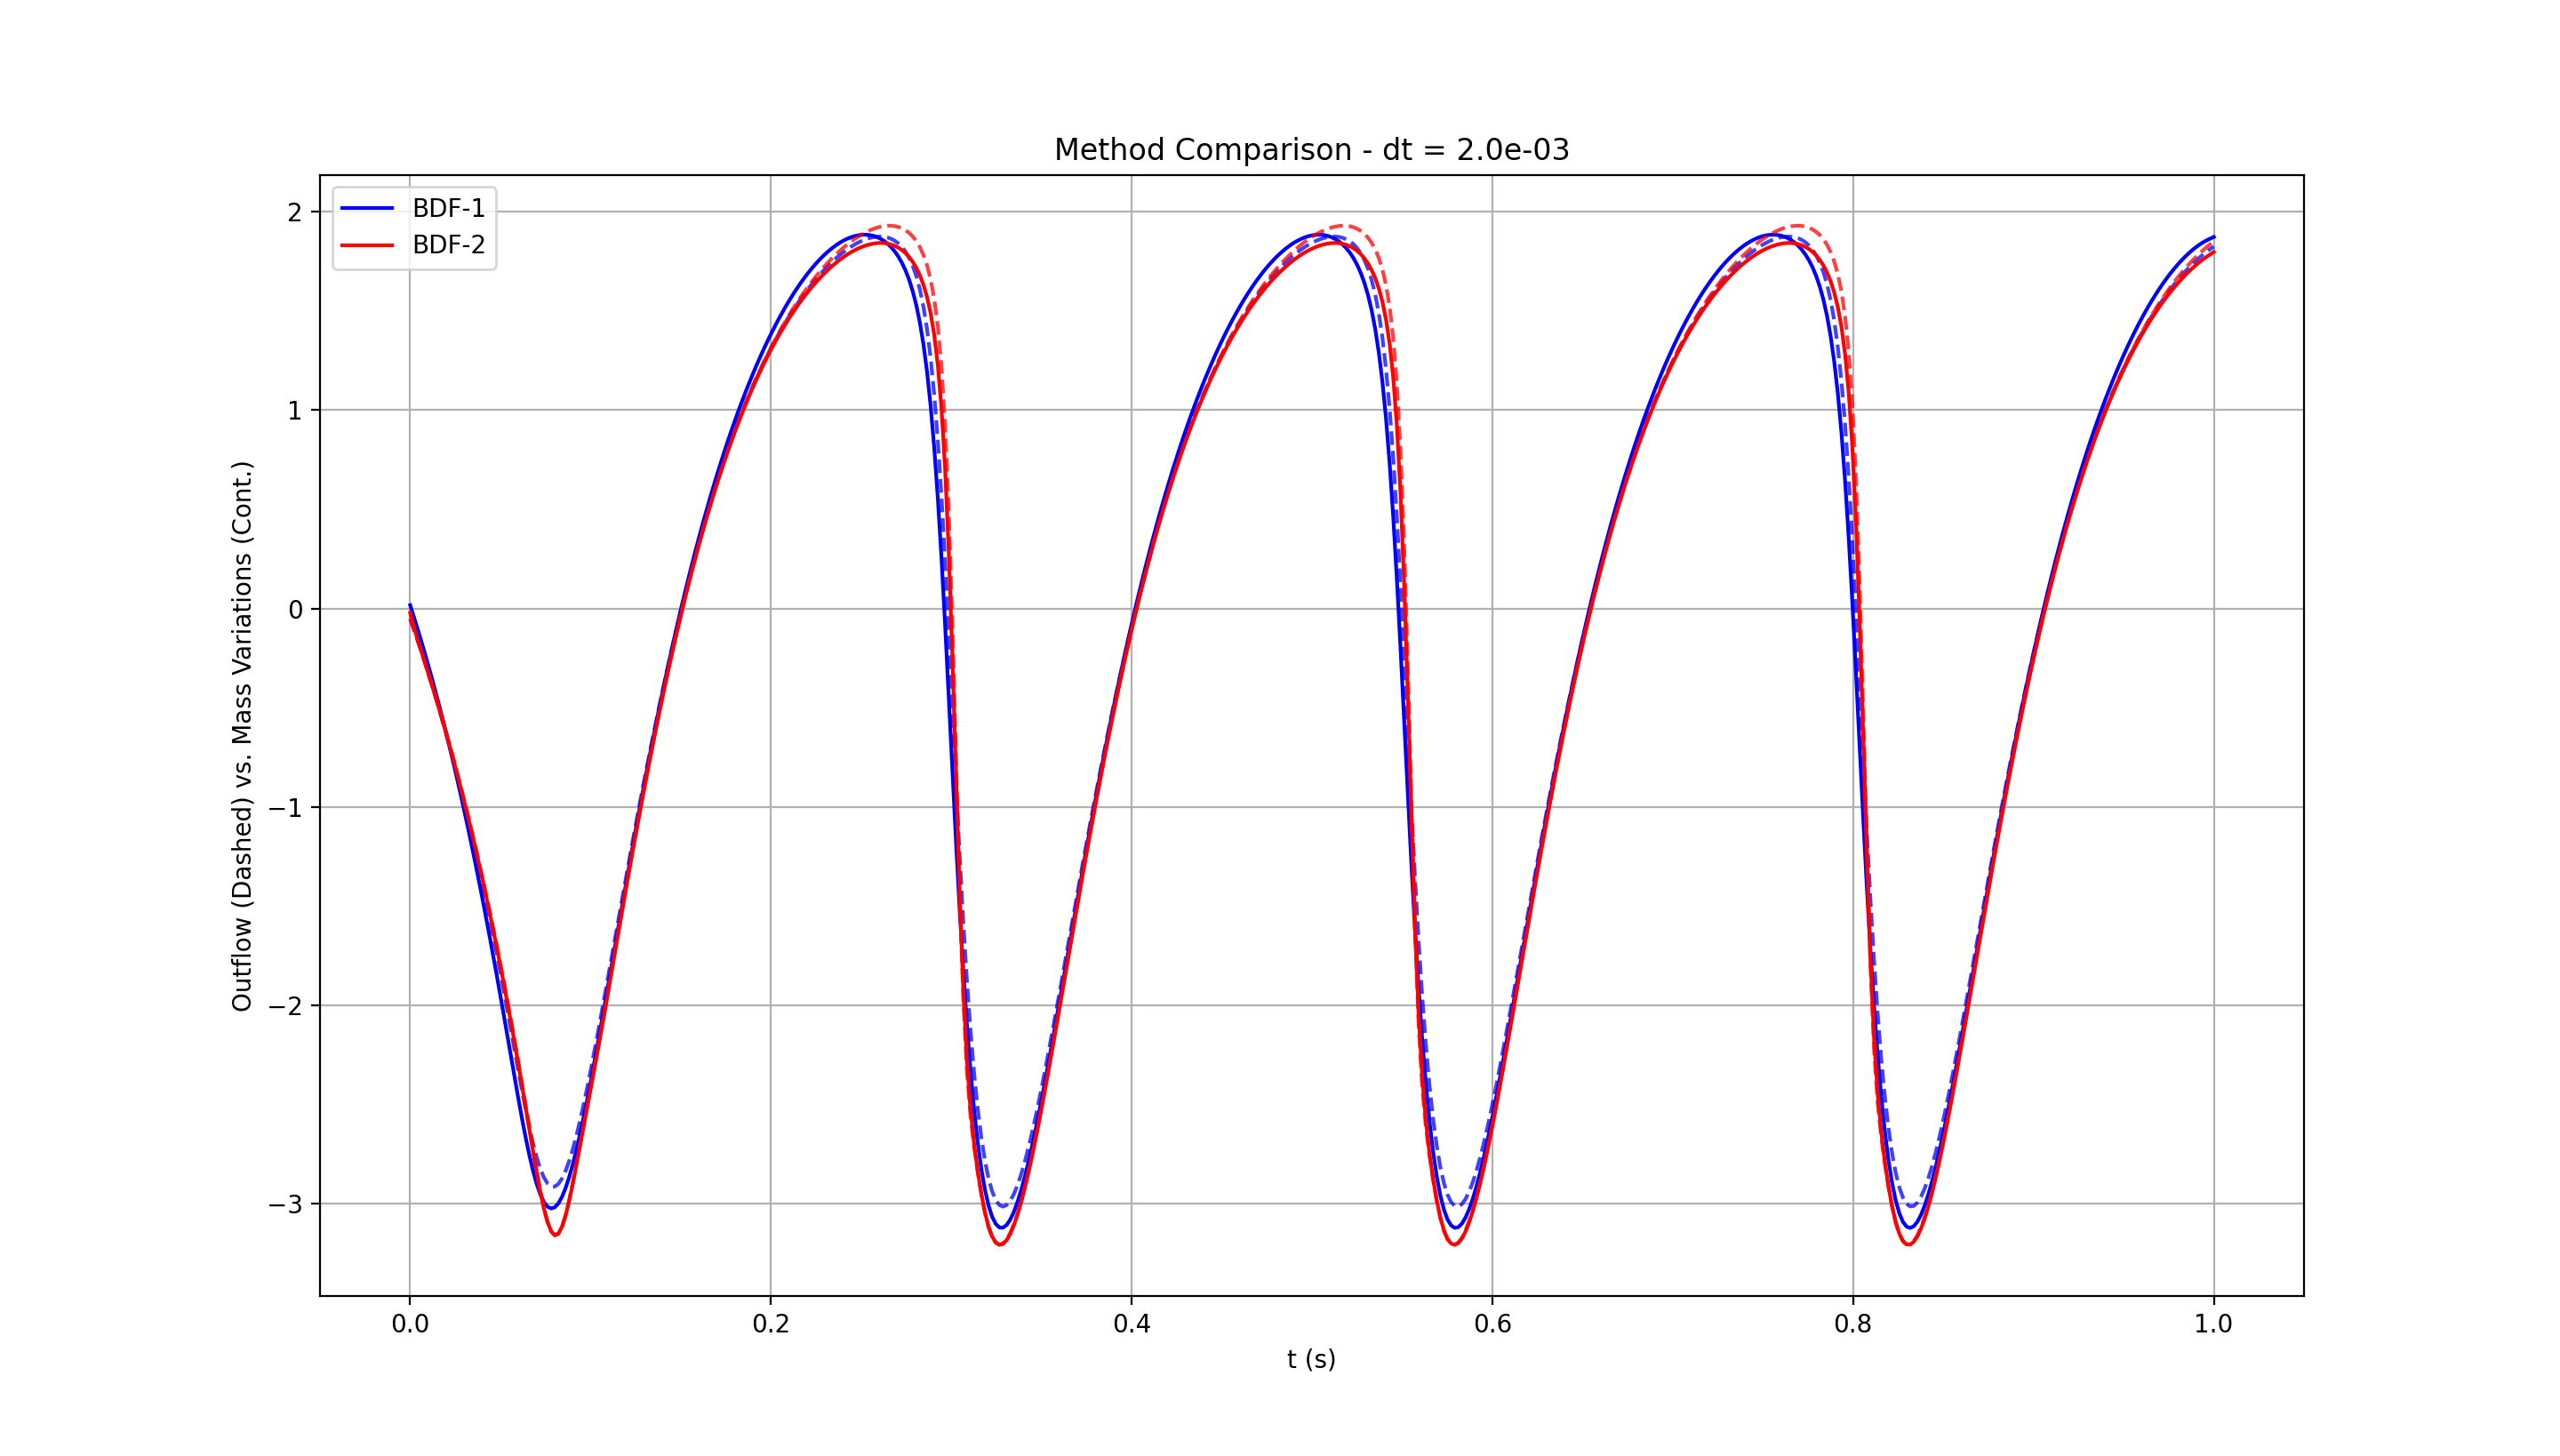
\includegraphics[width=\columnwidth]{research_project/piston/figures/consistency/mass_comparison.png}
%     \caption{Conservation of Mass, comparison between BDF-1 and BDF-2.
%     Cont.: $d/dt \int_{0}^{L(t)} \rho(x,t) dx$. 
%     Dashed: Outflow, $\rho(0,t)u(0,t)$.}
%     \label{fig:comparison_bdf}
% \end{figure}

% \begin{figure}[h]
%     \centering
%     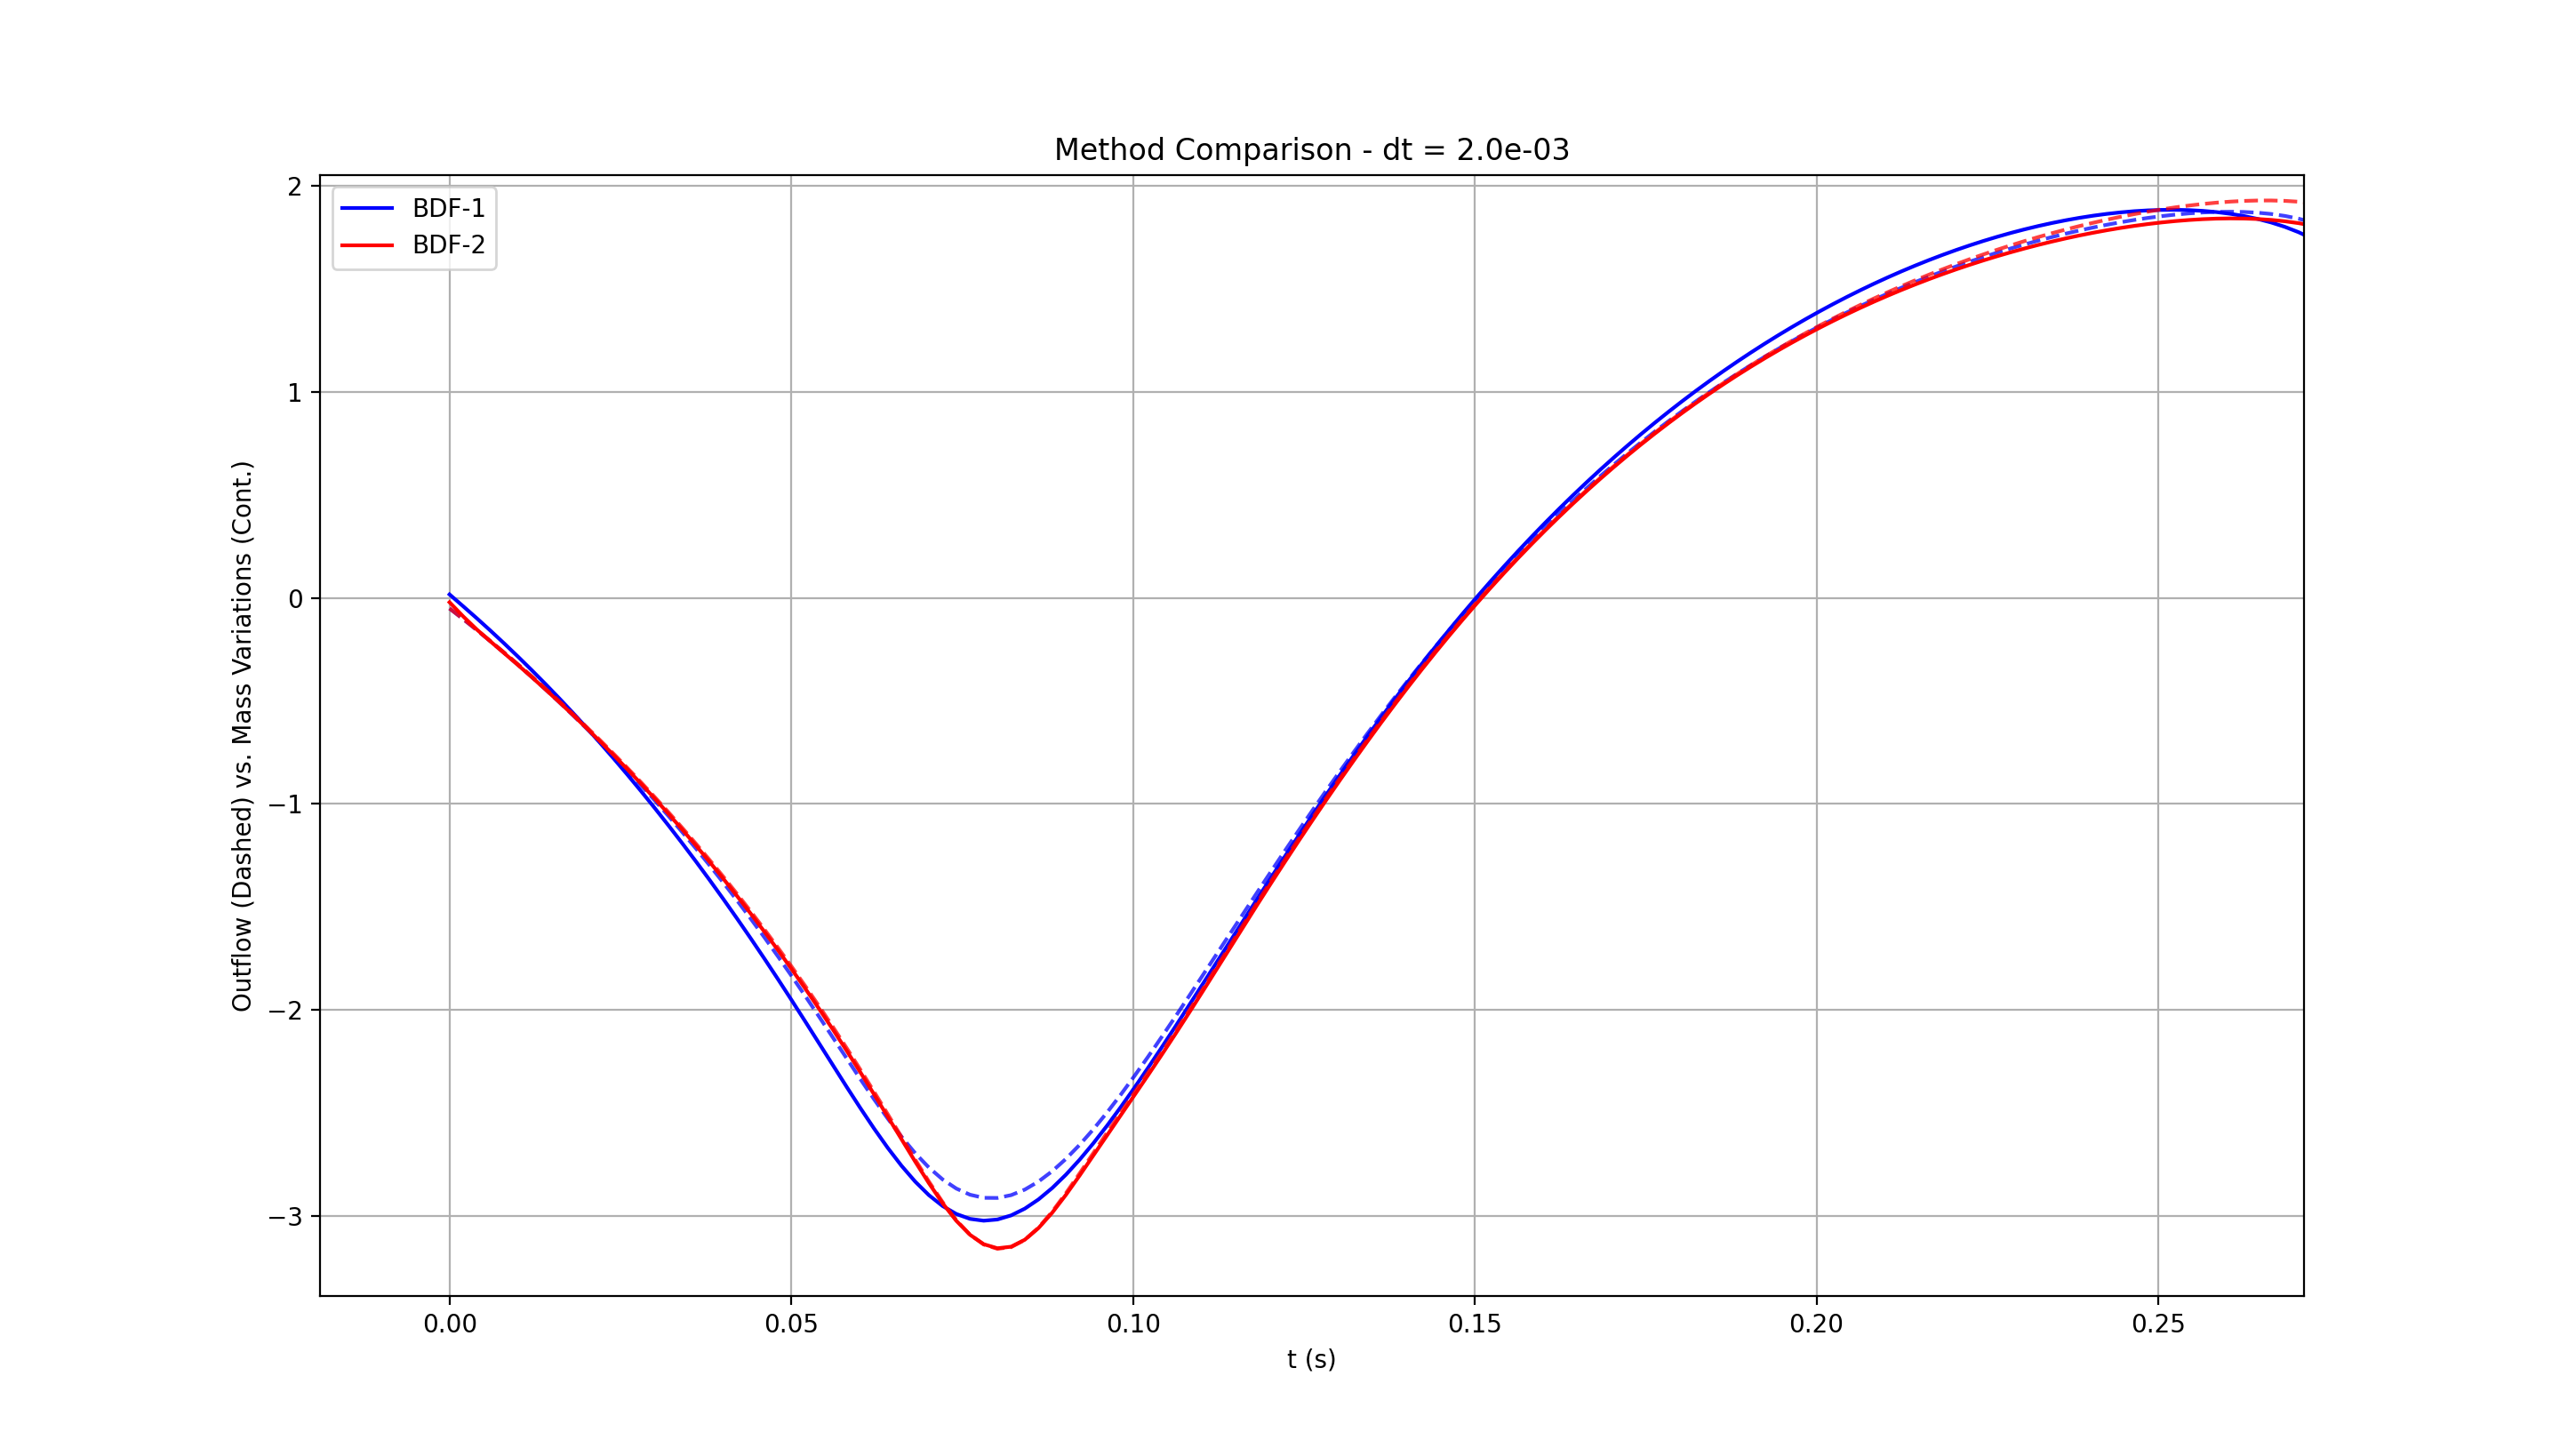
\includegraphics[width=\columnwidth]{research_project/piston/figures/consistency/mass_comparison_zoom.png}
%     \caption{Conservation of Mass, comparison between BDF-1 and BDF-2 (zoom).
%     Cont.: $d/dt \int_{0}^{L(t)} \rho(x,t) dx$. 
%     Dashed: Outflow, $\rho(0,t)u(0,t)$.}
%     \label{fig:comparison_bdf_zoom}
% \end{figure}

% \begin{figure}[h]
%     \centering
%     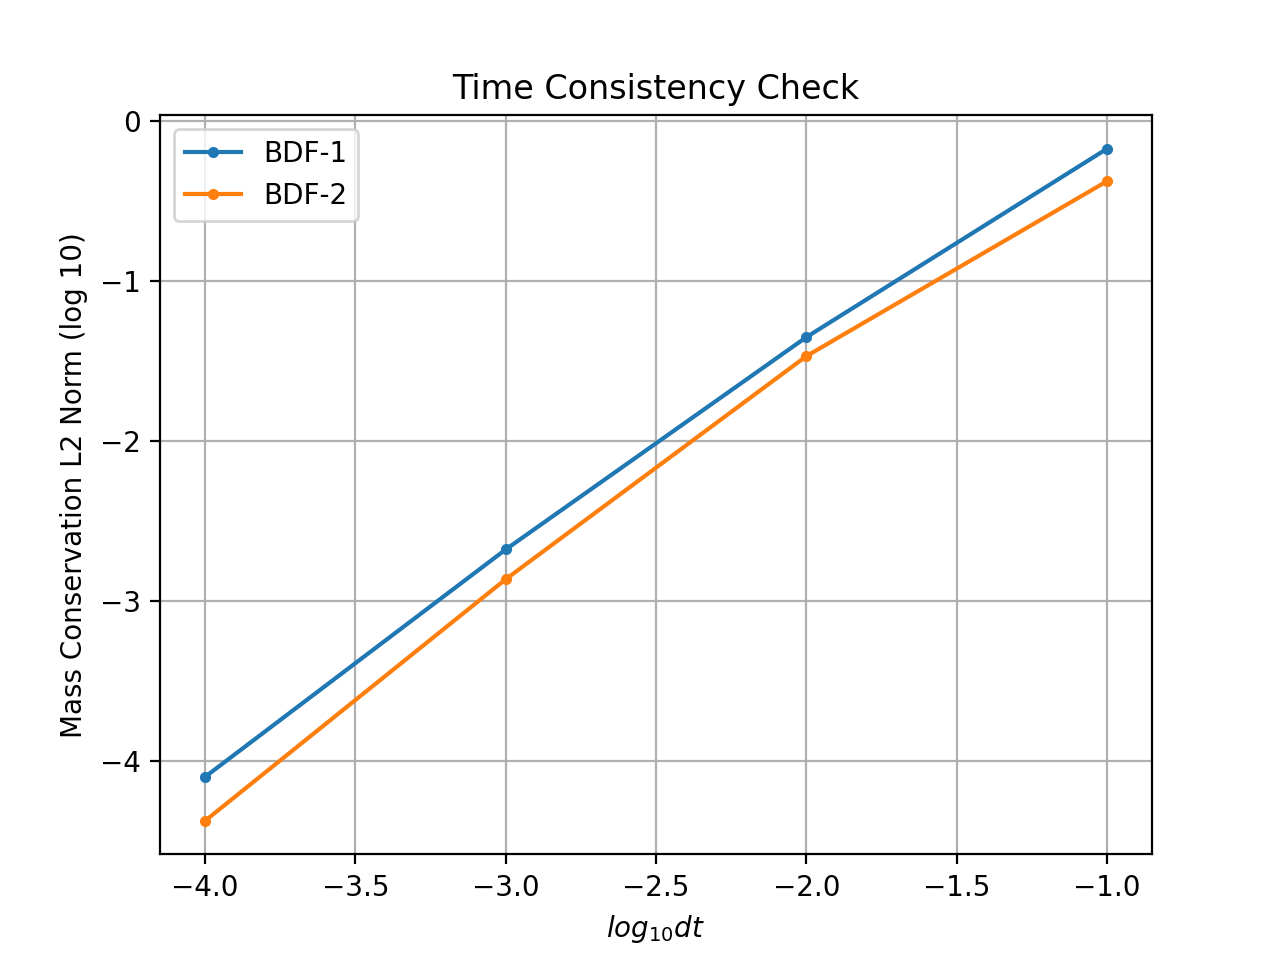
\includegraphics[width=\columnwidth]{research_project/piston/figures/consistency/l2_norm_vs_dt.png}
%     \caption{Conservation of Mass consistency.}
%     \label{fig:l2_vs_dt}
% \end{figure}

% \subsubsection{Conclusions}
% \begin{itemize}
%     \item The scheme seems consistent in the time variable, for the smaller we make the timestep, 
%     the smaller the error in the conservation of mass, as shown by Figure~\ref{fig:l2_vs_dt}.
%     \item Figures~\ref{fig:comparison_bdf} and \ref{fig:comparison_bdf_zoom} show a comparison between two time marching schemes.
%     The BDF-2 scheme seems to capture better the dynamics, for the only part where the outflow is different from the density time variation is near the upper peak. 
%     \item The fact that we do not see a slop of order two in Figure~\ref{fig:l2_vs_dt} could be due to the nature of the variable we are measuring, not necessarily a bug.
%         \begin{itemize}
%             \item According to Figure~\ref{fig:comparison_bdf_zoom}, the BDF-2 scheme captures better the dynamic of mass conservation.
%             \item The L2 errors is computed as the difference between outflow and mass variation, divided by $N_t$. 
%             I think that is the reason we see the same slope twice, because we are seeing $dt~\sim N_t^{-1}$ vs. $N_t^{-1}$
%             (and yet, the BDF-2 curve is underneath the BDF-1). 
%         \end{itemize}
% \end{itemize}

% \newpage
% \newpage
% \subsection{System Approximation: DEIM and MDEIM}
% Due to the simplicity of the geometry (1D piston), the linear operators are reduced effortlessly.
% We recall that to build the collateral space (the basis for the algebraic operators), we are using a nested POD approach:
% \begin{enumerate}
%     \item Select parameter, assemble in time, compress, collect basis.
%     \item Update parameter, repeat assembly and compression in time.
%     \item Compress all the collected basis for each parameter.
% \end{enumerate}

% % Please add the following required packages to your document preamble:
% % \usepackage{booktabs}
% \begin{table}[h]
%     \caption{Number of basis after the tree walk (collection of basis per parameter) and the final basis size once the final POD is applied.
%     Five parameters were sampled for the offline phase of the collateral basis.}
%     \begin{tabular}{@{}rcc@{}}
%     \toprule
%                       & basis-shape-after-tree-walk & basis-shape-final \\ \midrule
%     mass              & 5                           & 1                 \\
%     stiffness         & 5                           & 1                 \\
%     convection        & 10                          & 2                 \\
%     nonlinear-lifting & 5                           & 1                 \\
%     rhs               & 12                          & 4                 \\ \midrule
%     nonlinear         & 90                          & 18                \\
%     nonlinear         & 465                         & 93                \\ \bottomrule
%     \end{tabular}
%     \label{tab:summary_basis_deim}
% \end{table}
% As we can see in Table~\ref{tab:summary_basis_deim}, linear operators can be resolved by a few number of basis.
% This is so because their main nonlinearity is the implicit jacobian which is present due to the time-dependency of the domain.
% Since it is a very simple domain (1D piston), the jacobian is a function of time and space,
% \begin{equation}
%     J \sim L'(t) x,
% \end{equation}
% so its reduction is immediate. 

% The RHS requires a bit more of terms because it contains the action of all the operators unto the lifting function.

% \subsubsection{Nonlinear term}
% To assemble the nonlinear term, we use the reduced basis modes as a proxy for the actual solution which is used in the discretization.
% This is a fair approach, since eventually the solution will be a linear combination of such modes.
% Thus, the number of basis after the tree walk depends not only in the number of parameters, but also in the number of reduced basis elements.
% Again, a three-level nested POD approach is used:
% \begin{enumerate}
%     \item For a given parameter, for each timestep:
%     \begin{enumerate}
%         \item Assemble for each basis element, compress, collect.
%         \item Update time, repeat assemly and compression in reduced basis space.
%     \end{enumerate}
%     \item Update parameter, repeat assembly and compression in time.
%     \item Compress all the collected basis for each parameter.
% \end{enumerate}
% A very decent reduction ratio can be achieved.

% \subsubsection{Online errors}
% With the collateral basis, we sample unseen parameters and assemble the operators to evaluate our collateral basis.
% As expected given the simplicity of the implicit nonlinearity, they are reconstruced to machine accuracy, as shown 
% in Figures~\ref{fig:online_rhs}, \ref{fig:online_mass_errors}, \ref{fig:online_stiffness_errors}, \ref{fig:online_convection_errors}, 
% \ref{fig:online_nonlinear_lifting_errors},
% \ref{fig:online_nonlinear_errors_tol} and
% \ref{fig:online_nonlinear_errors_full}. 
% \begin{figure}[p]
%     \centering
%     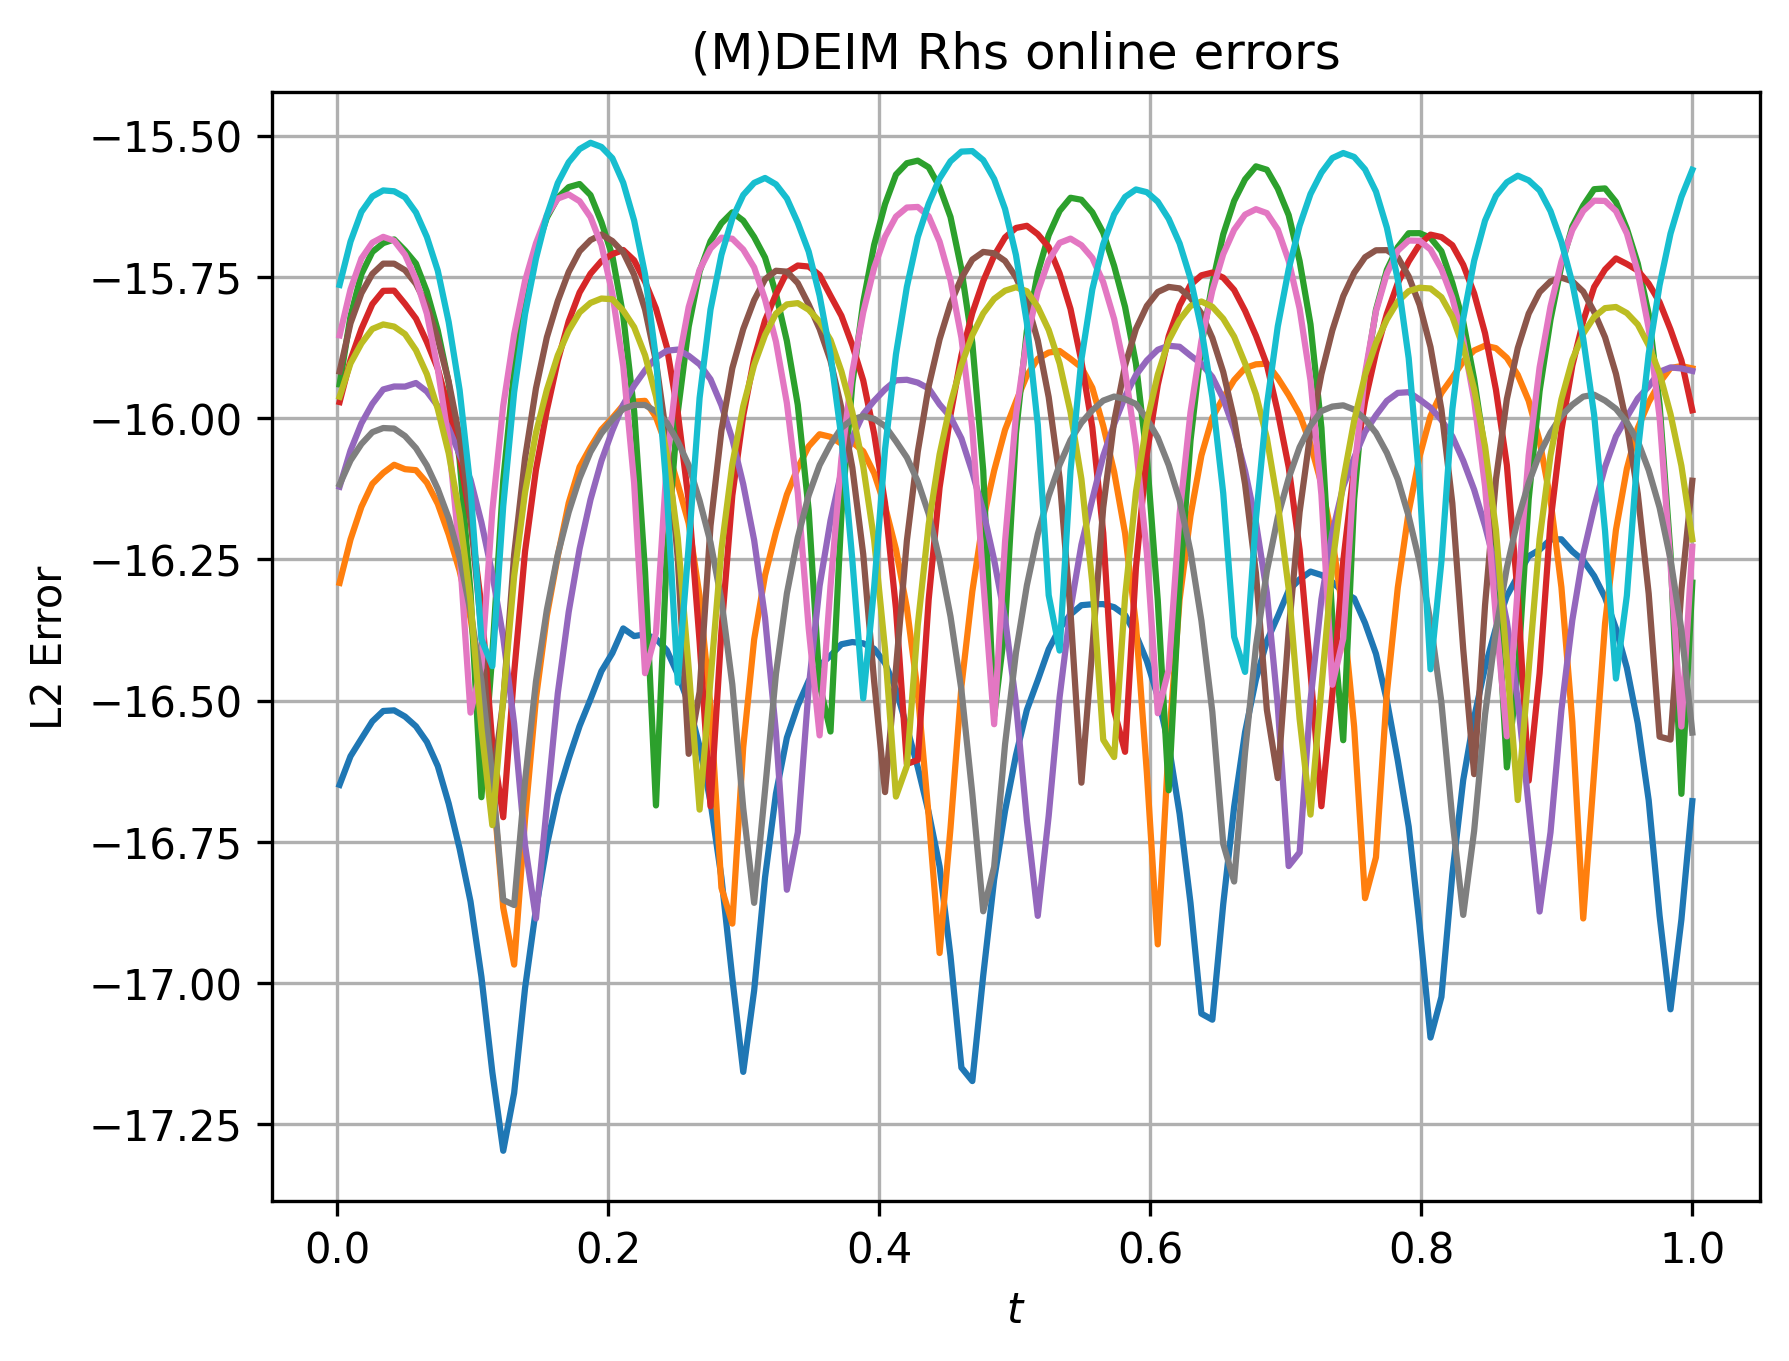
\includegraphics[width=\columnwidth]{research_project/piston/figures/hrom/deim_errors/mdeim_RHS_online_errors.png}
%     \caption{Online errors: Rhs functional.}
%     \label{fig:online_rhs}
% \end{figure}
% \begin{figure}[p]
%     \centering
%     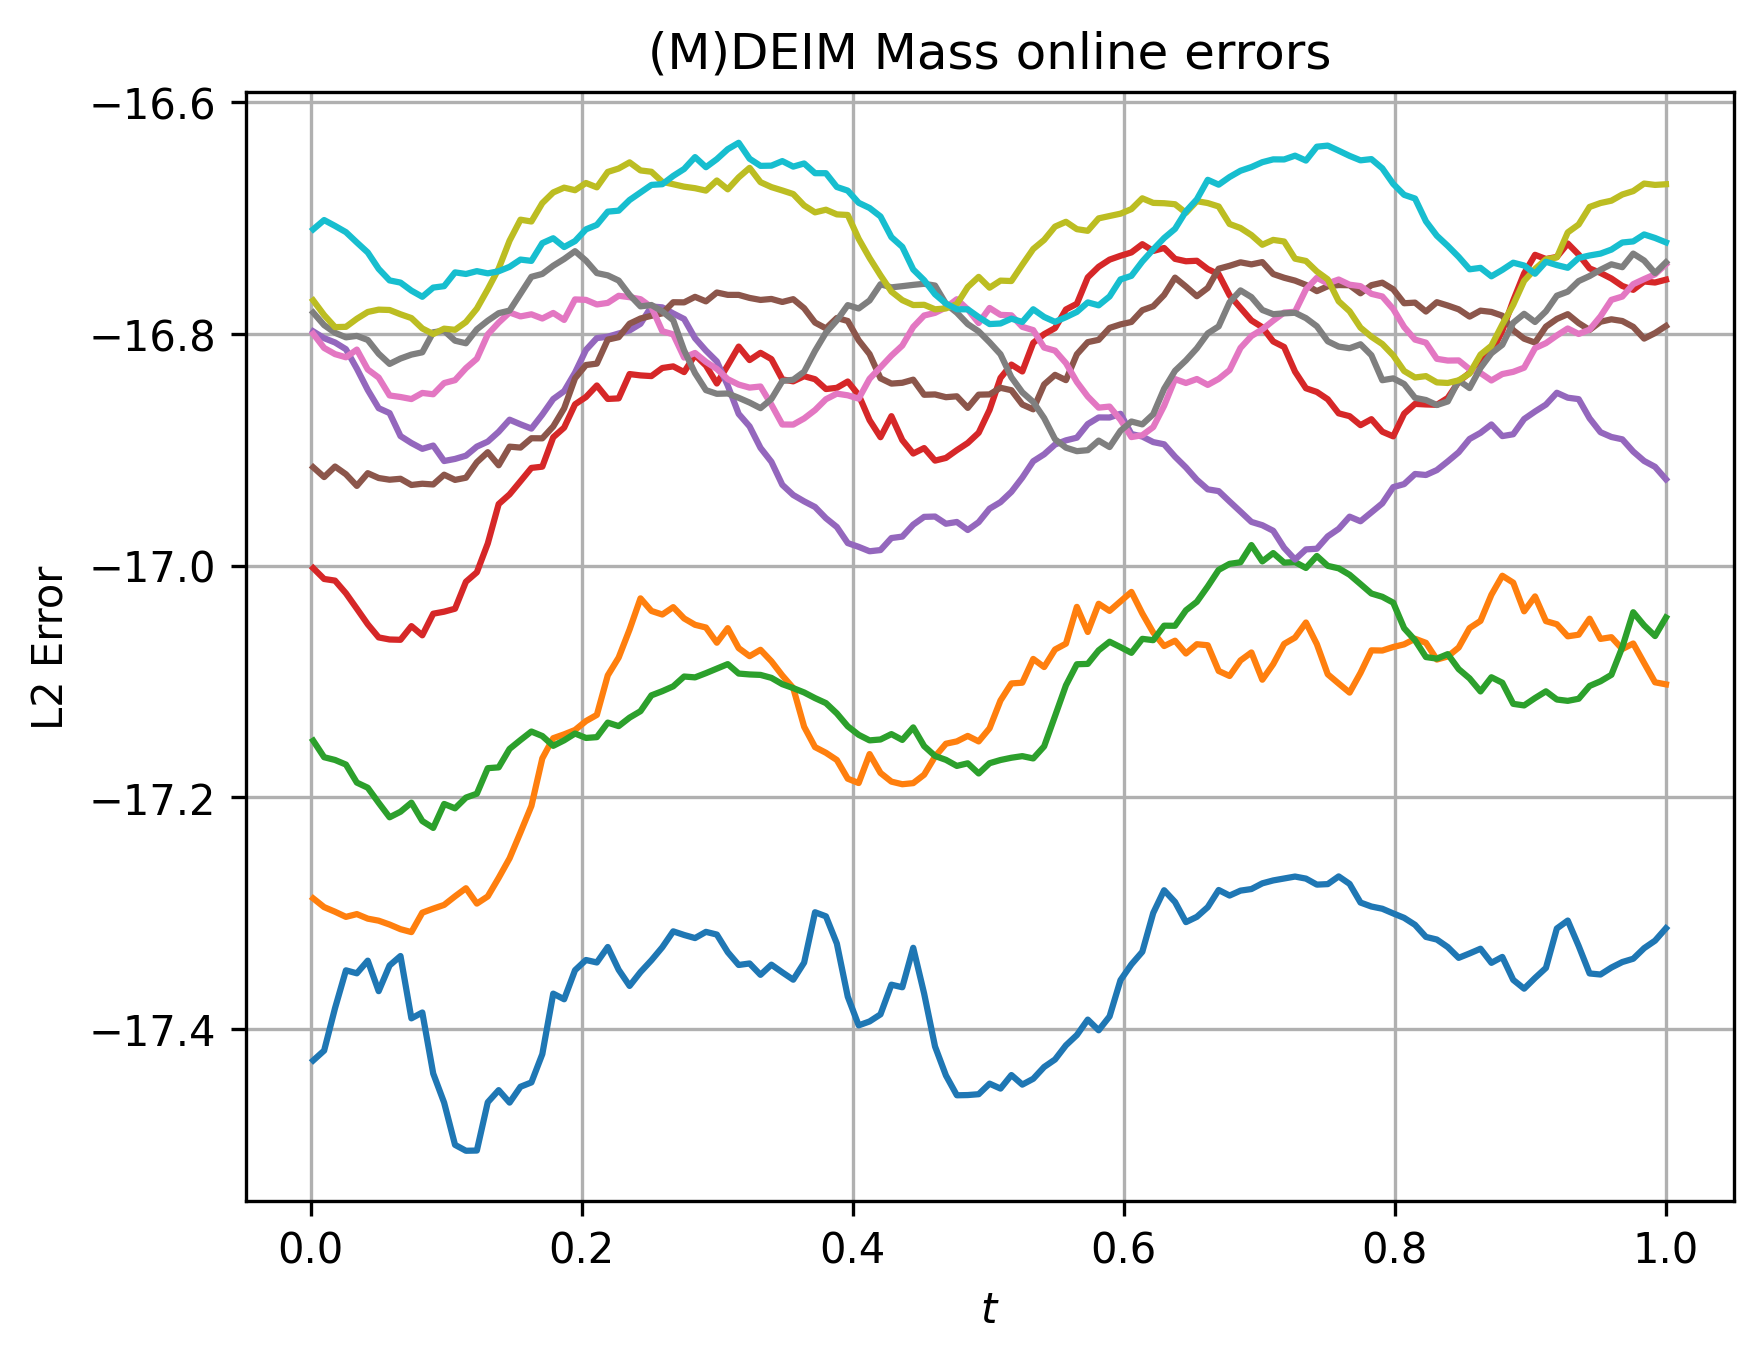
\includegraphics[width=\columnwidth]{research_project/piston/figures/hrom/deim_errors/mdeim_Mass_online_errors.png}
%     \caption{Online errors: mass operator.}
%     \label{fig:online_mass_errors}
% \end{figure}
% \begin{figure}[p]
%     \centering
%     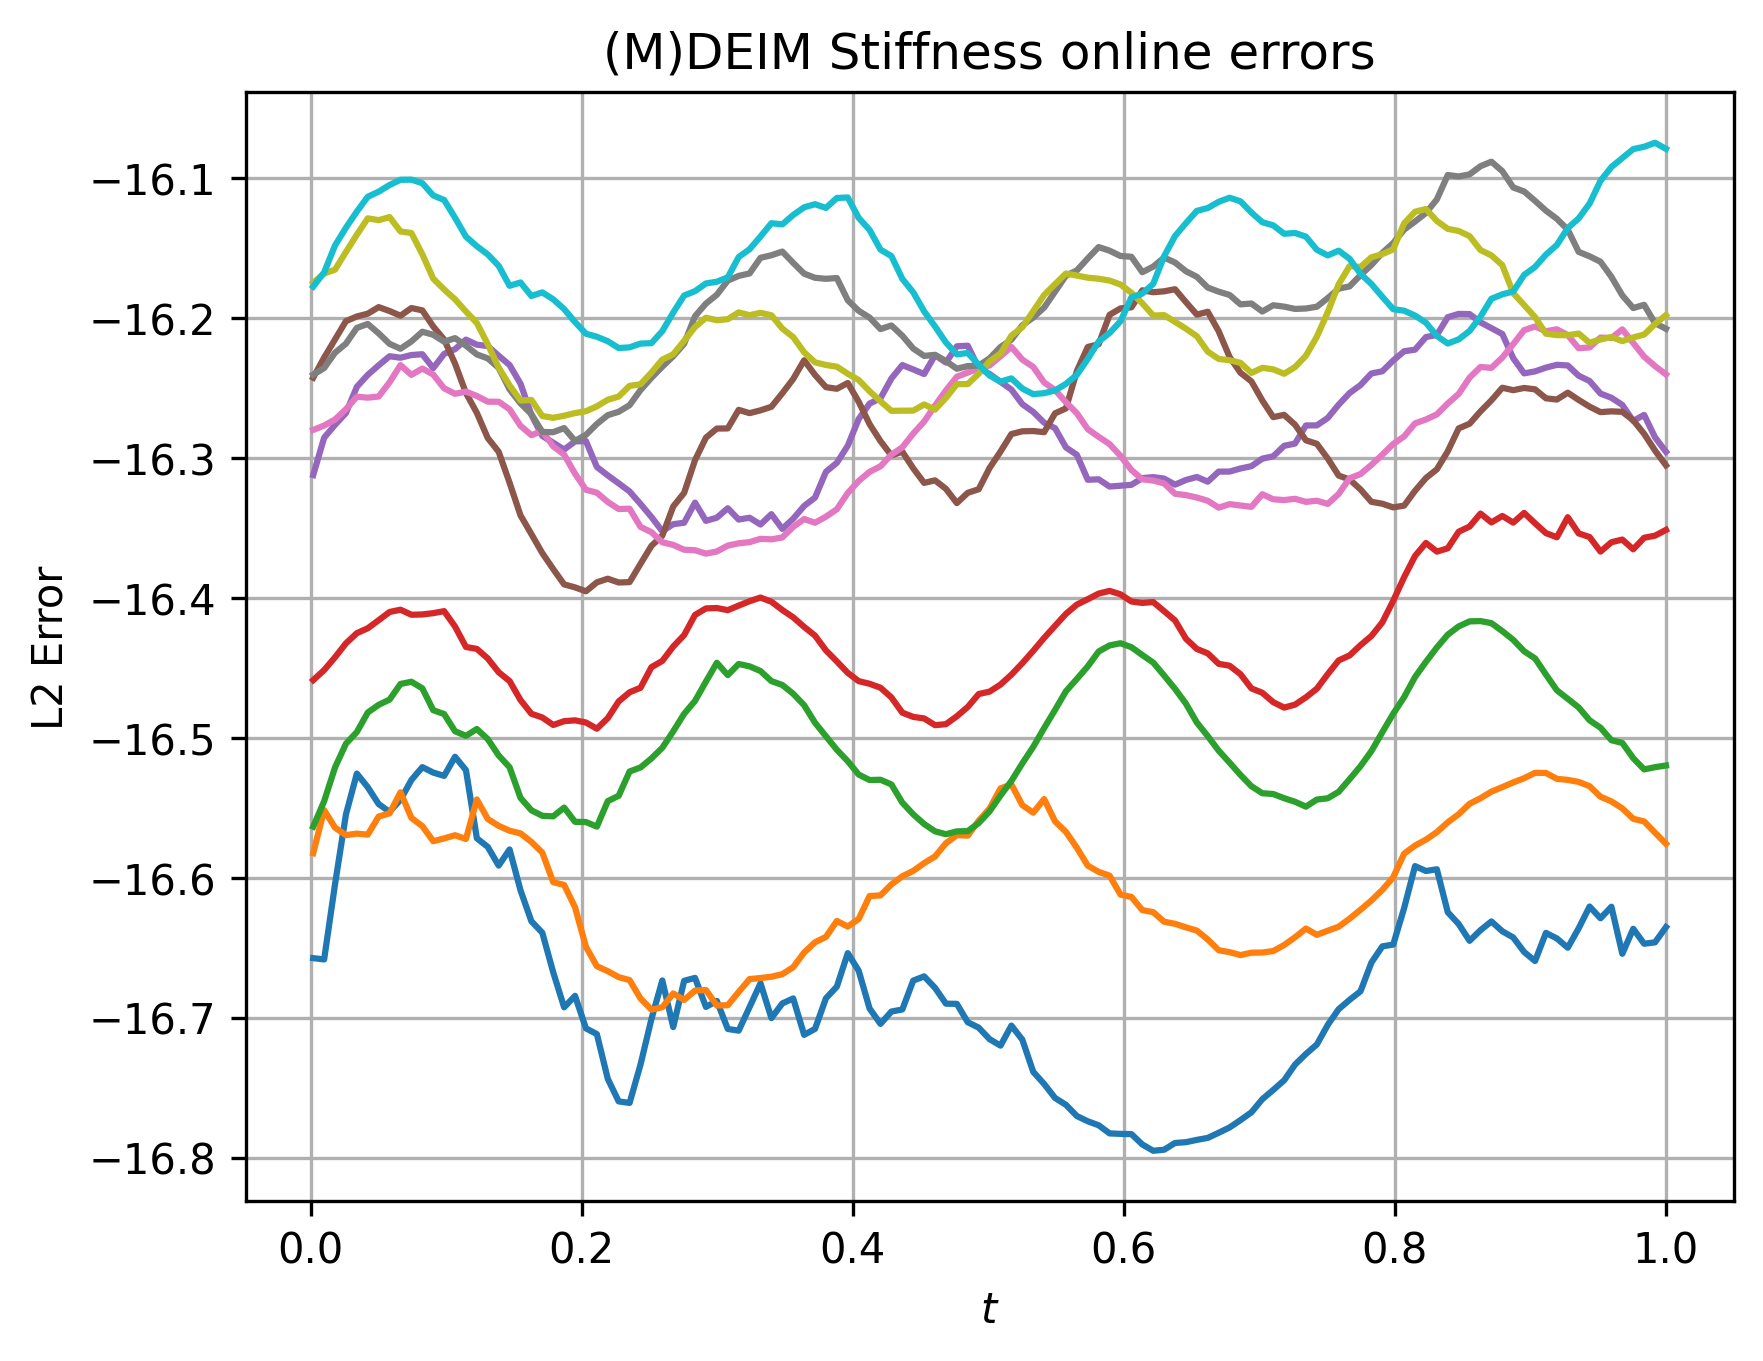
\includegraphics[width=\columnwidth]{research_project/piston/figures/hrom/deim_errors/mdeim_Stiffness_online_errors.png}
%     \caption{Online errors: stiffness operator.}
%     \label{fig:online_stiffness_errors}
% \end{figure}
% \begin{figure}[p]
%     \centering
%     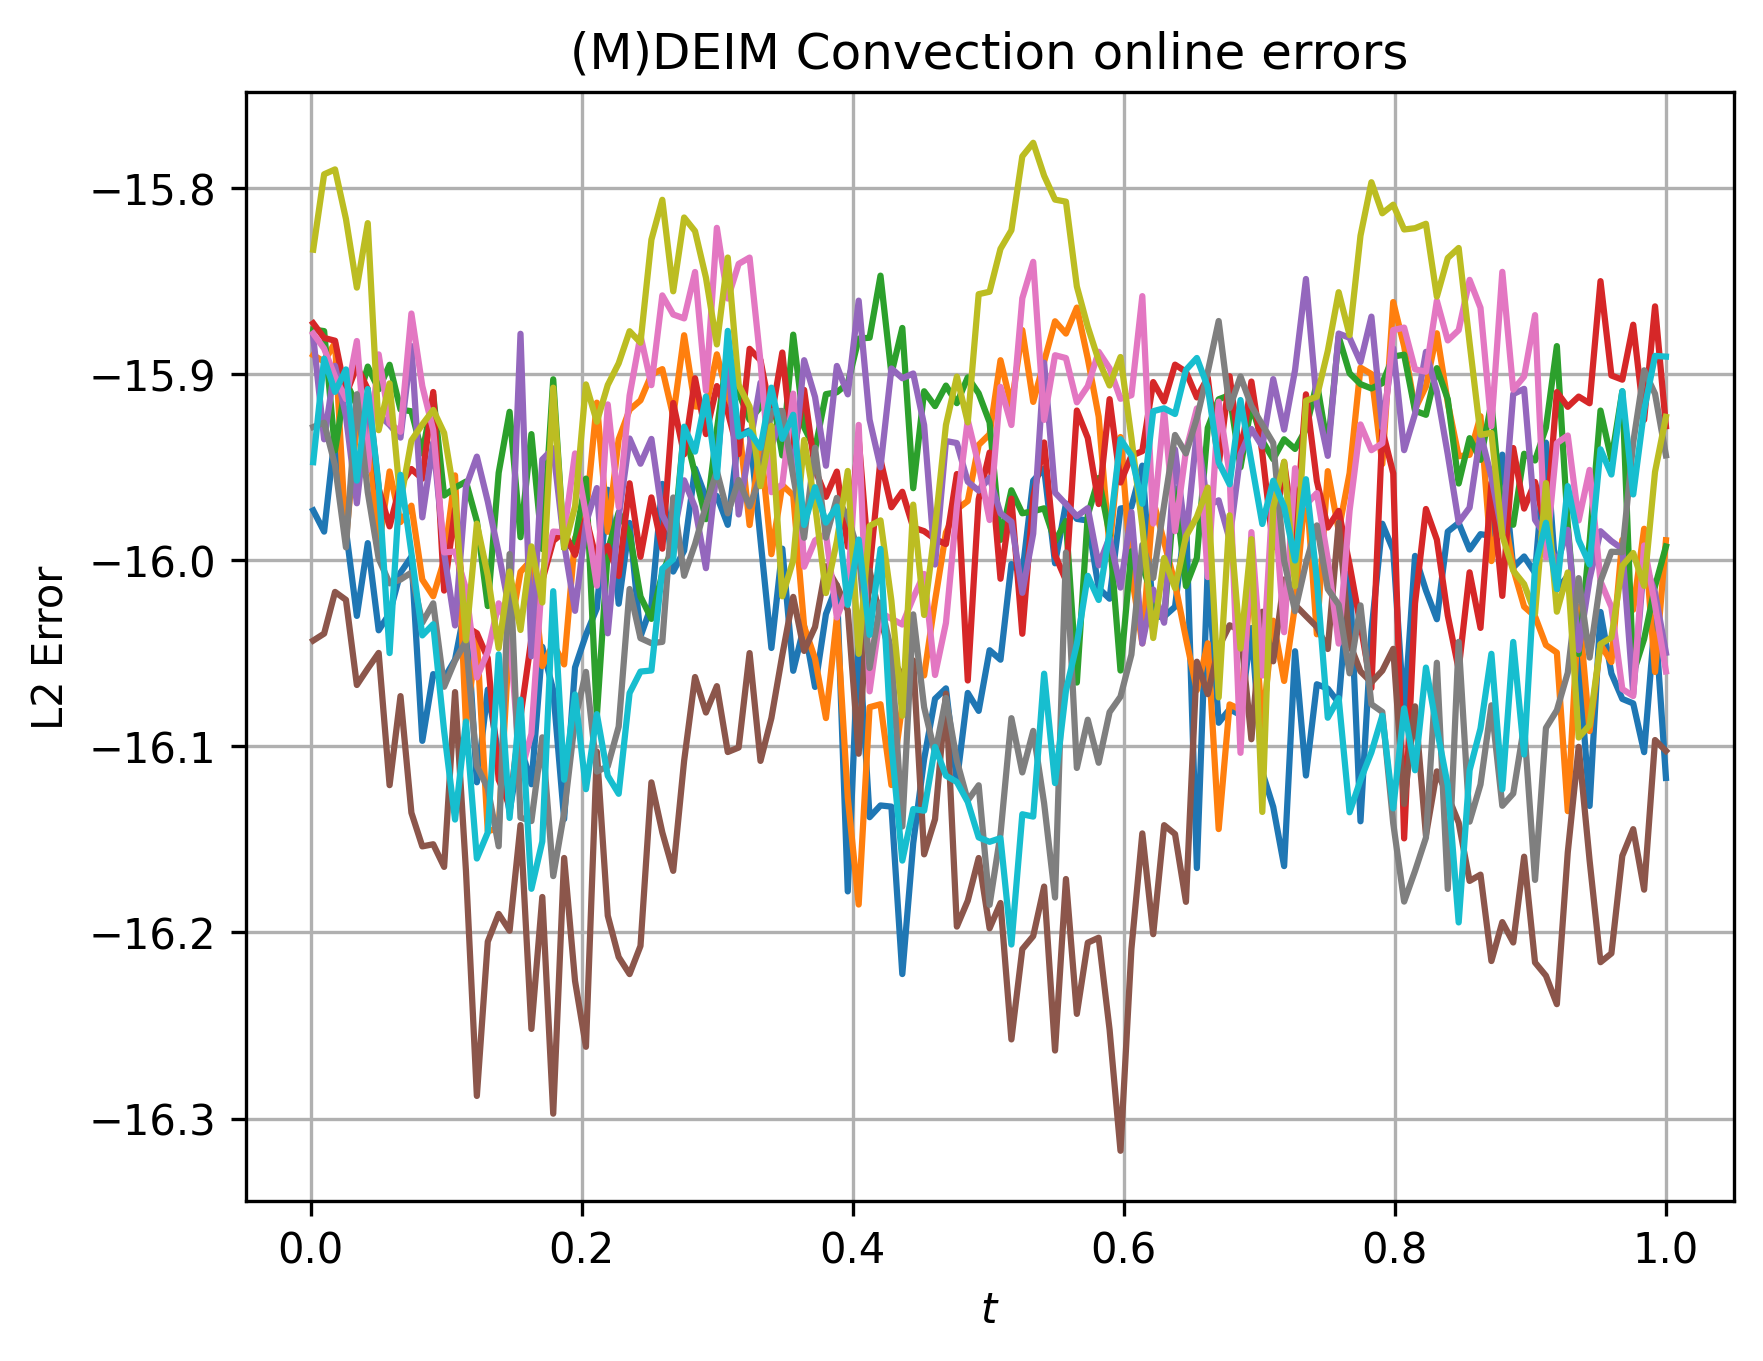
\includegraphics[width=\columnwidth]{research_project/piston/figures/hrom/deim_errors/mdeim_convection_online_errors.png}
%     \caption{Online errors: convection operator. It contains the speed of sound and the ALE velocity.}
%     \label{fig:online_convection_errors}
% \end{figure}
% \begin{figure}[p]
%     \centering
%     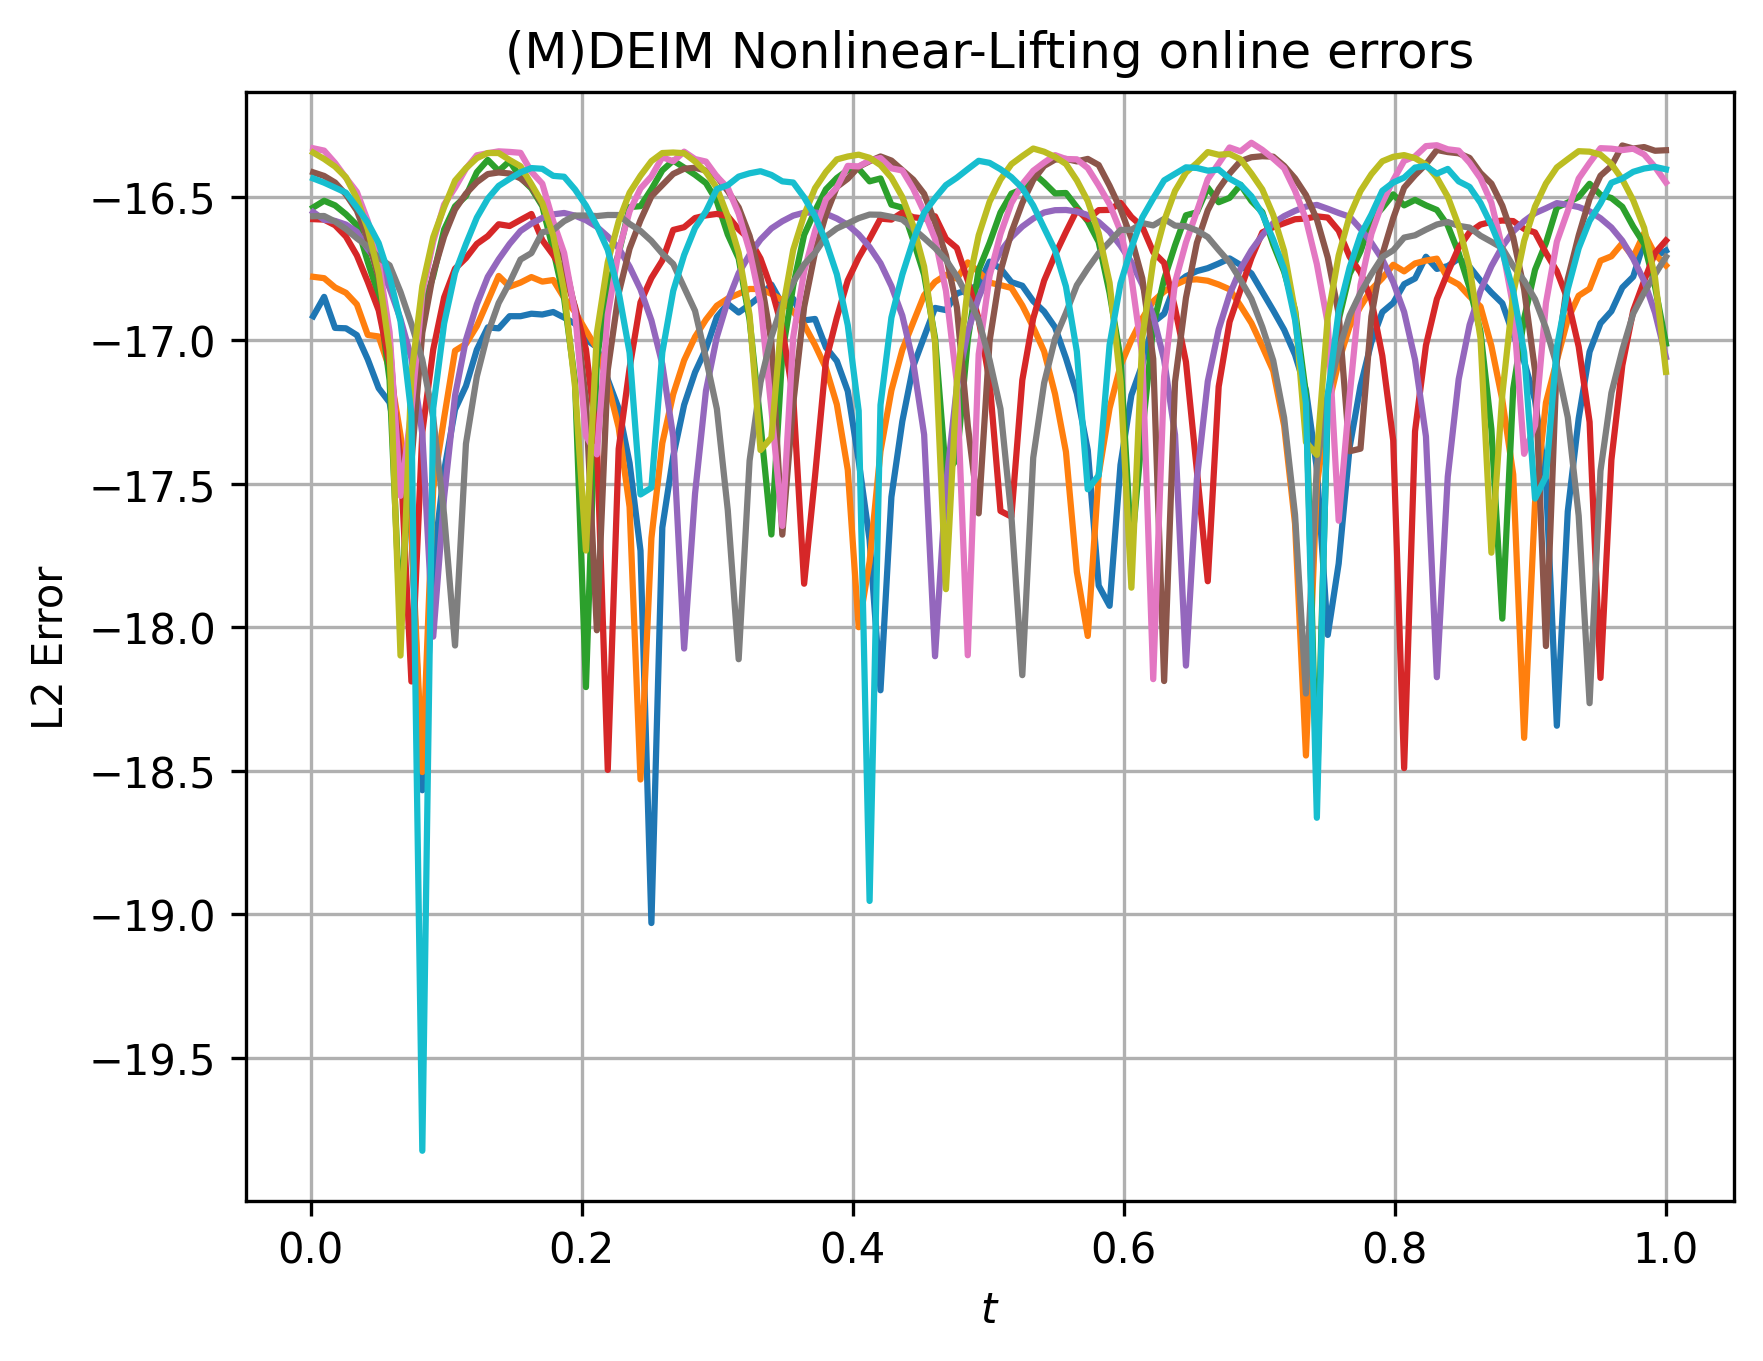
\includegraphics[width=\columnwidth]{research_project/piston/figures/hrom/deim_errors/mdeim_nonlinear-lifting_online_errors.png}
%     \caption{Online errors: nonlinear lifting operator (it is the linearized nonlinear operator).}
%     \label{fig:online_nonlinear_lifting_errors}
% \end{figure}
% \begin{figure}[p]
%     \centering
%     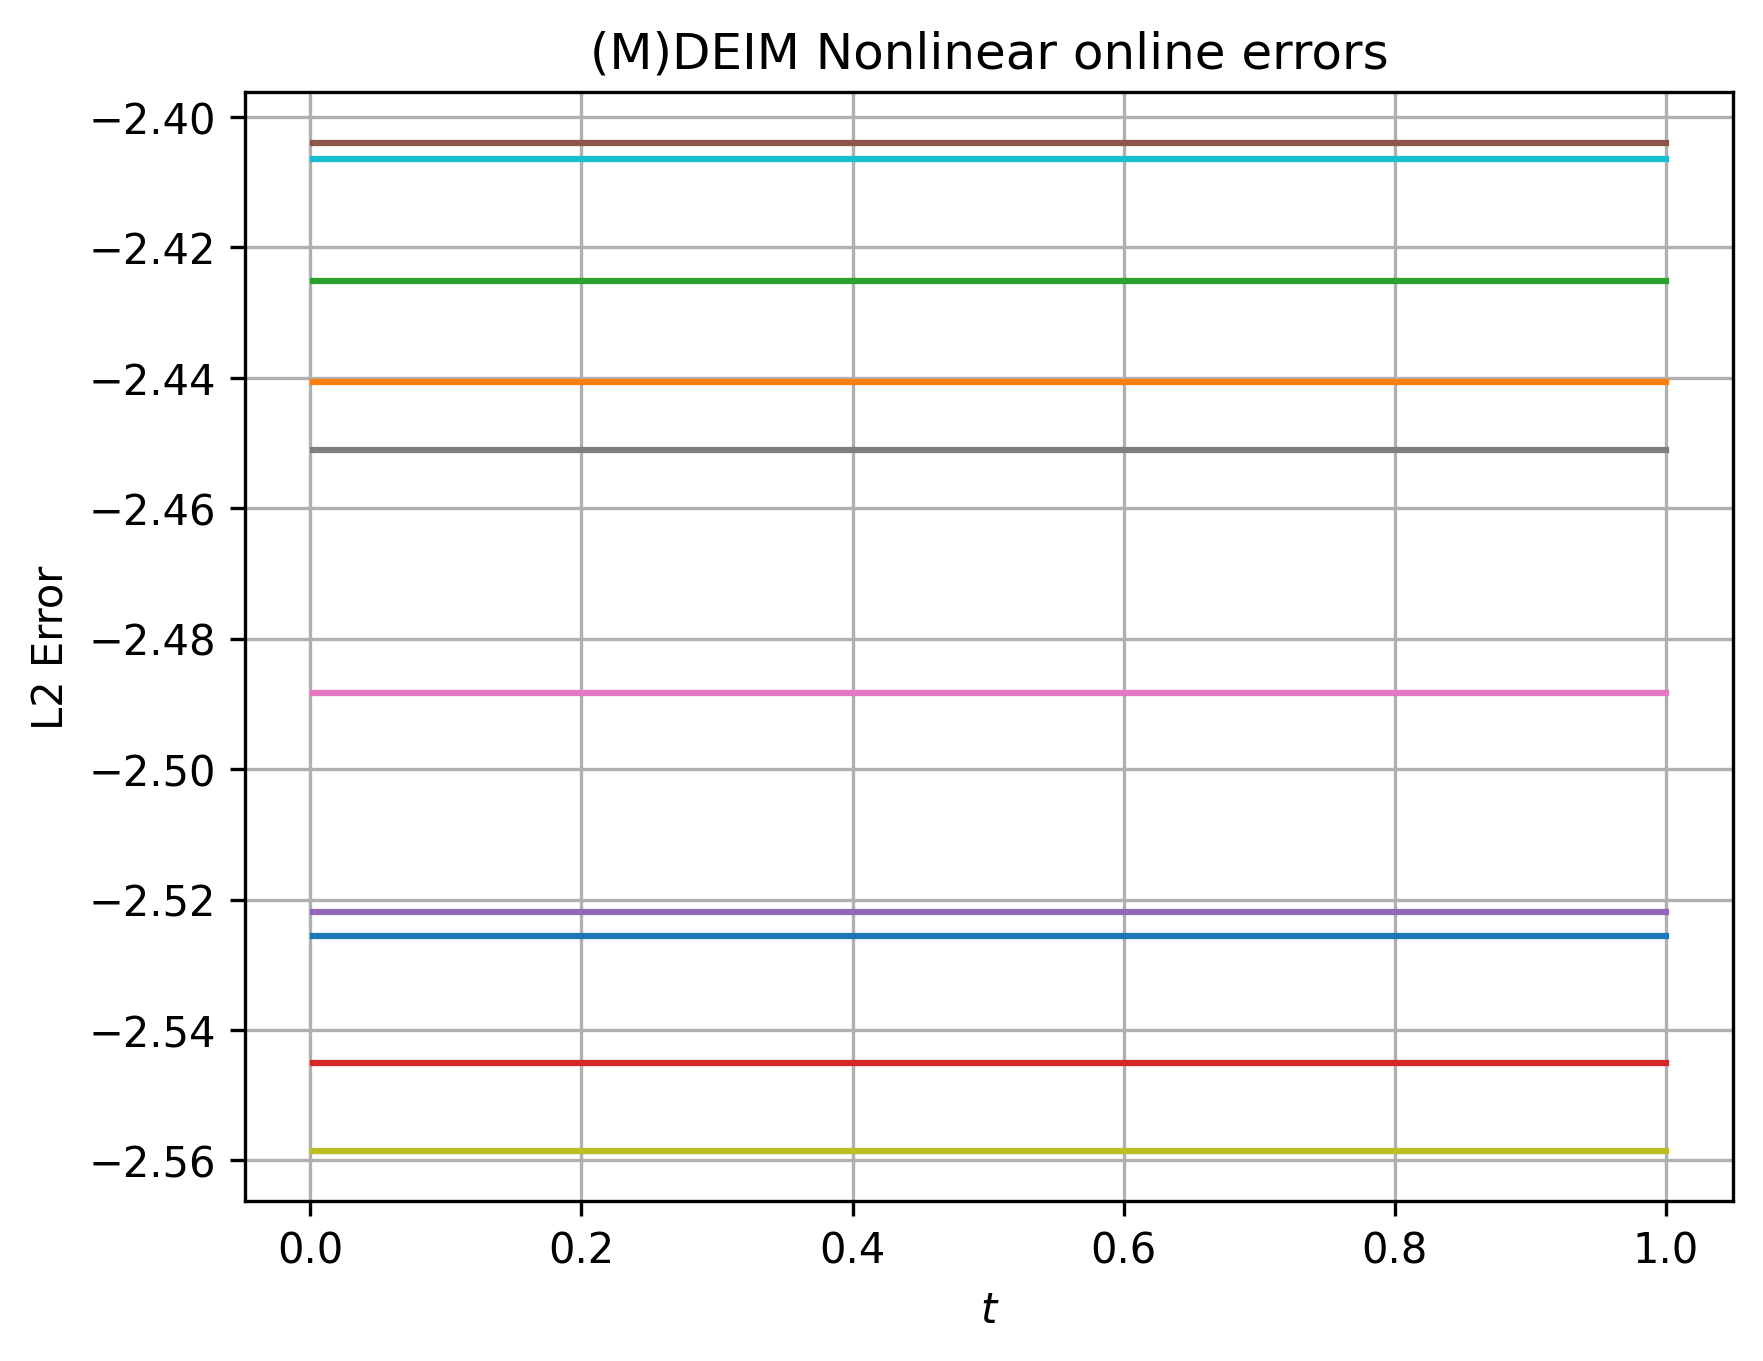
\includegraphics[width=\columnwidth]{research_project/piston/figures/hrom/deim_errors/mdeim_nonlinear_tol.png}
%     \caption{Online errors: nonlinear operator with 50\%-energy basis, poor reconstruction.}
%     \label{fig:online_nonlinear_errors_tol}
% \end{figure}
% \begin{figure}[p]
%     \centering
%     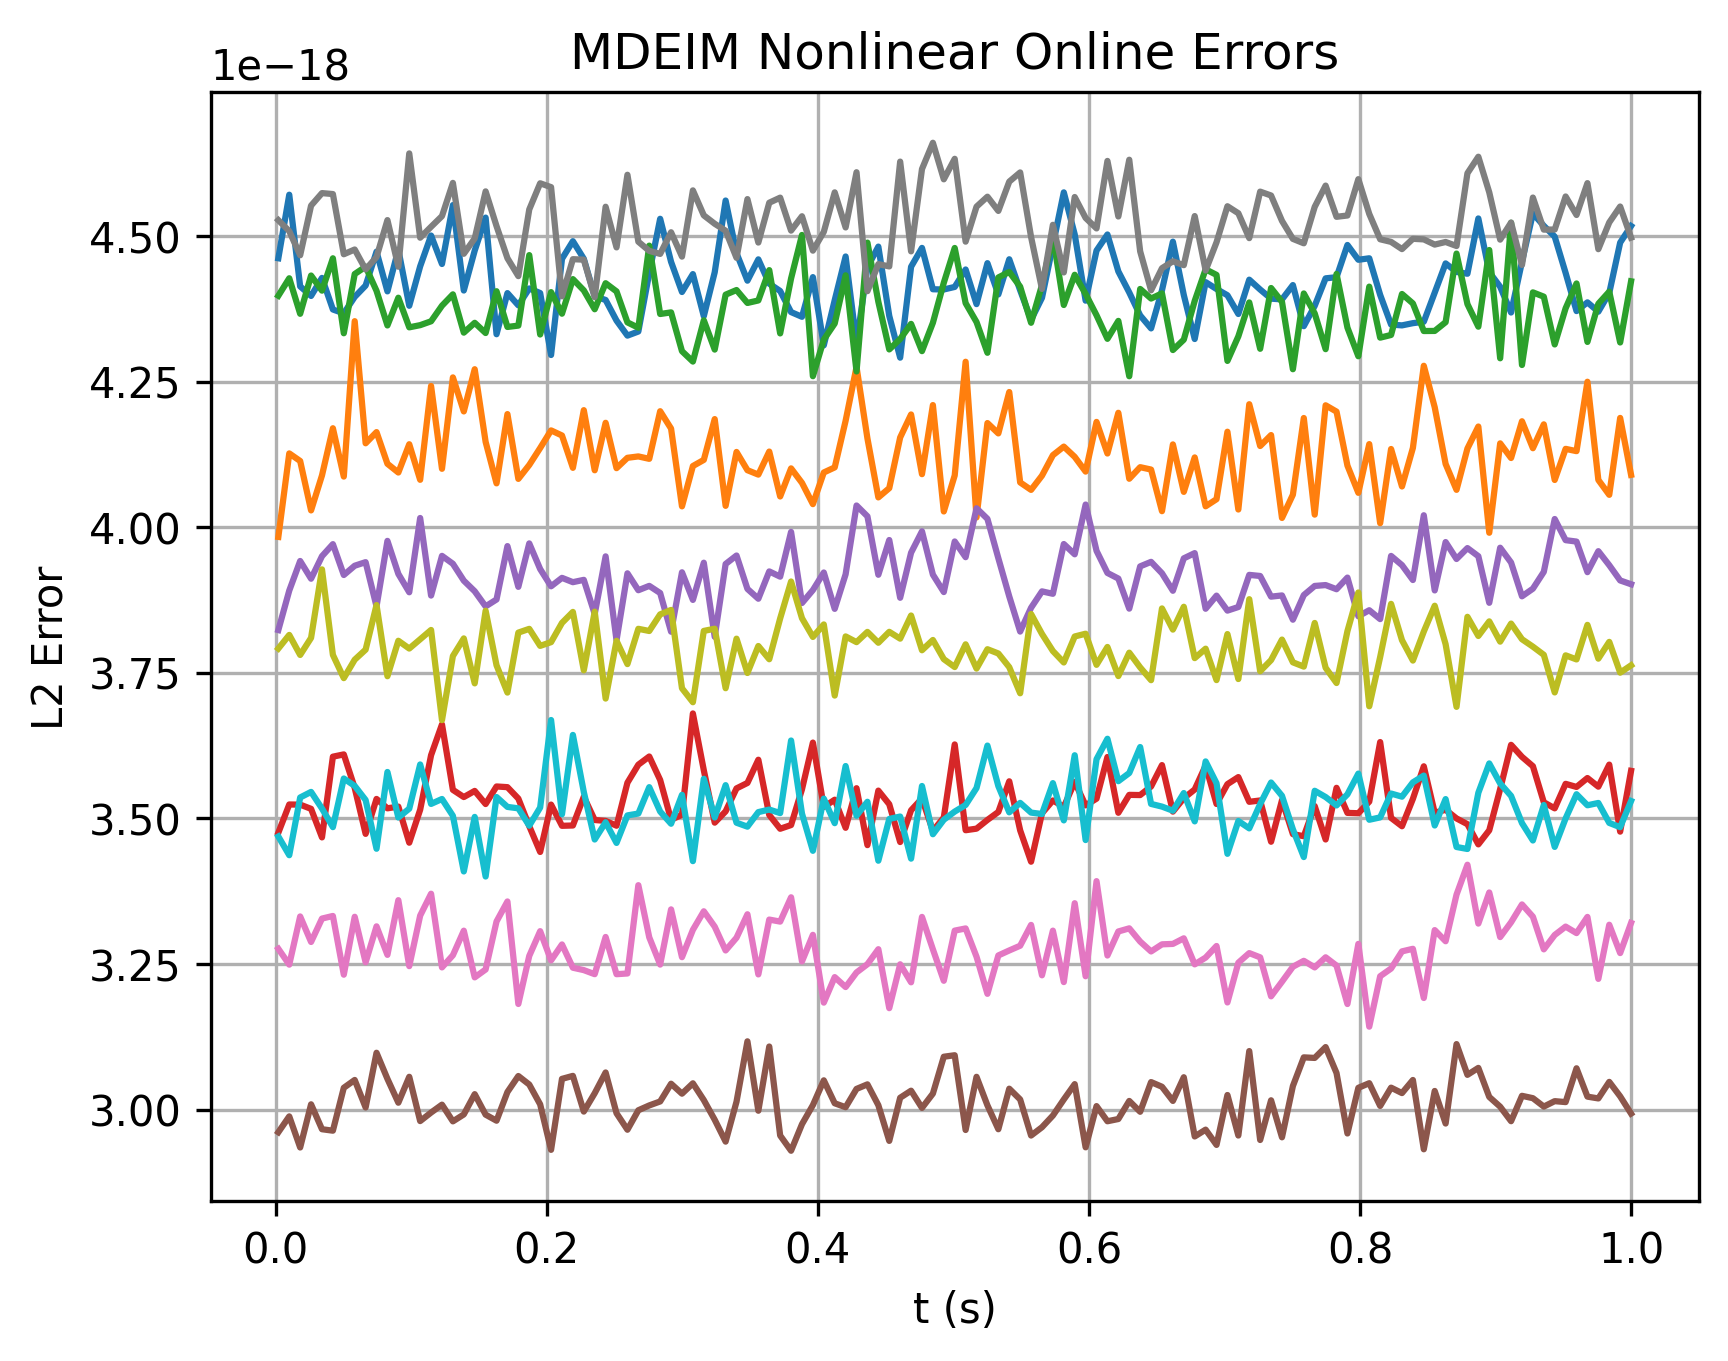
\includegraphics[width=\columnwidth]{research_project/piston/figures/hrom/deim_errors/mdeim_nonlinear_full.png}
%     \caption{Online errors: nonlinear operator with full basis. Exact reconstruction.}
%     \label{fig:online_nonlinear_errors_full}
% \end{figure}

% \newpage
% \newpage
% \subsection{Model Reduction: Tolerances in the Parameter Space}
% We recall that to build the reduced space, we are using a nested POD approach:
% \begin{itemize}
%     \item Select parameter, solve in time, compress, collect basis.
%     \item Update parameter, repeat solution and compression in time.
%     \item Compress all the collected basis for each parameter.
% \end{itemize}
% All the parameters are selected probing an uniformly distributed random variable, see Figure~\ref{fig:mu_space}.

% We ran three tests:
% \begin{enumerate}
%     \item \textbf{Benchmark}: automatic basis selection, all basis elements whose singular values are $\sigma > 10^{-7}$ are kept.
%     This is the most complete reduced basis one can get.
%     \item \textbf{Half-Space} (Fix tolerance in the parameter space for the solution and the nonlinear term): 
%     we keep all the basis elements which explain up 50\% of the variance. This is a strong reduction criteria.
%     \item \textbf{Reduced Solution Space}: we keep the automatic basis selection for the collateral basis (algebraic operators) 
%     and maintain the 50\% criteria for the reduced basis. 
% \end{enumerate}
% For each of them we ran the ROM unto the training parameter set and the online set, which was never seen before.

% \begin{figure}[p]
%     \centering
%     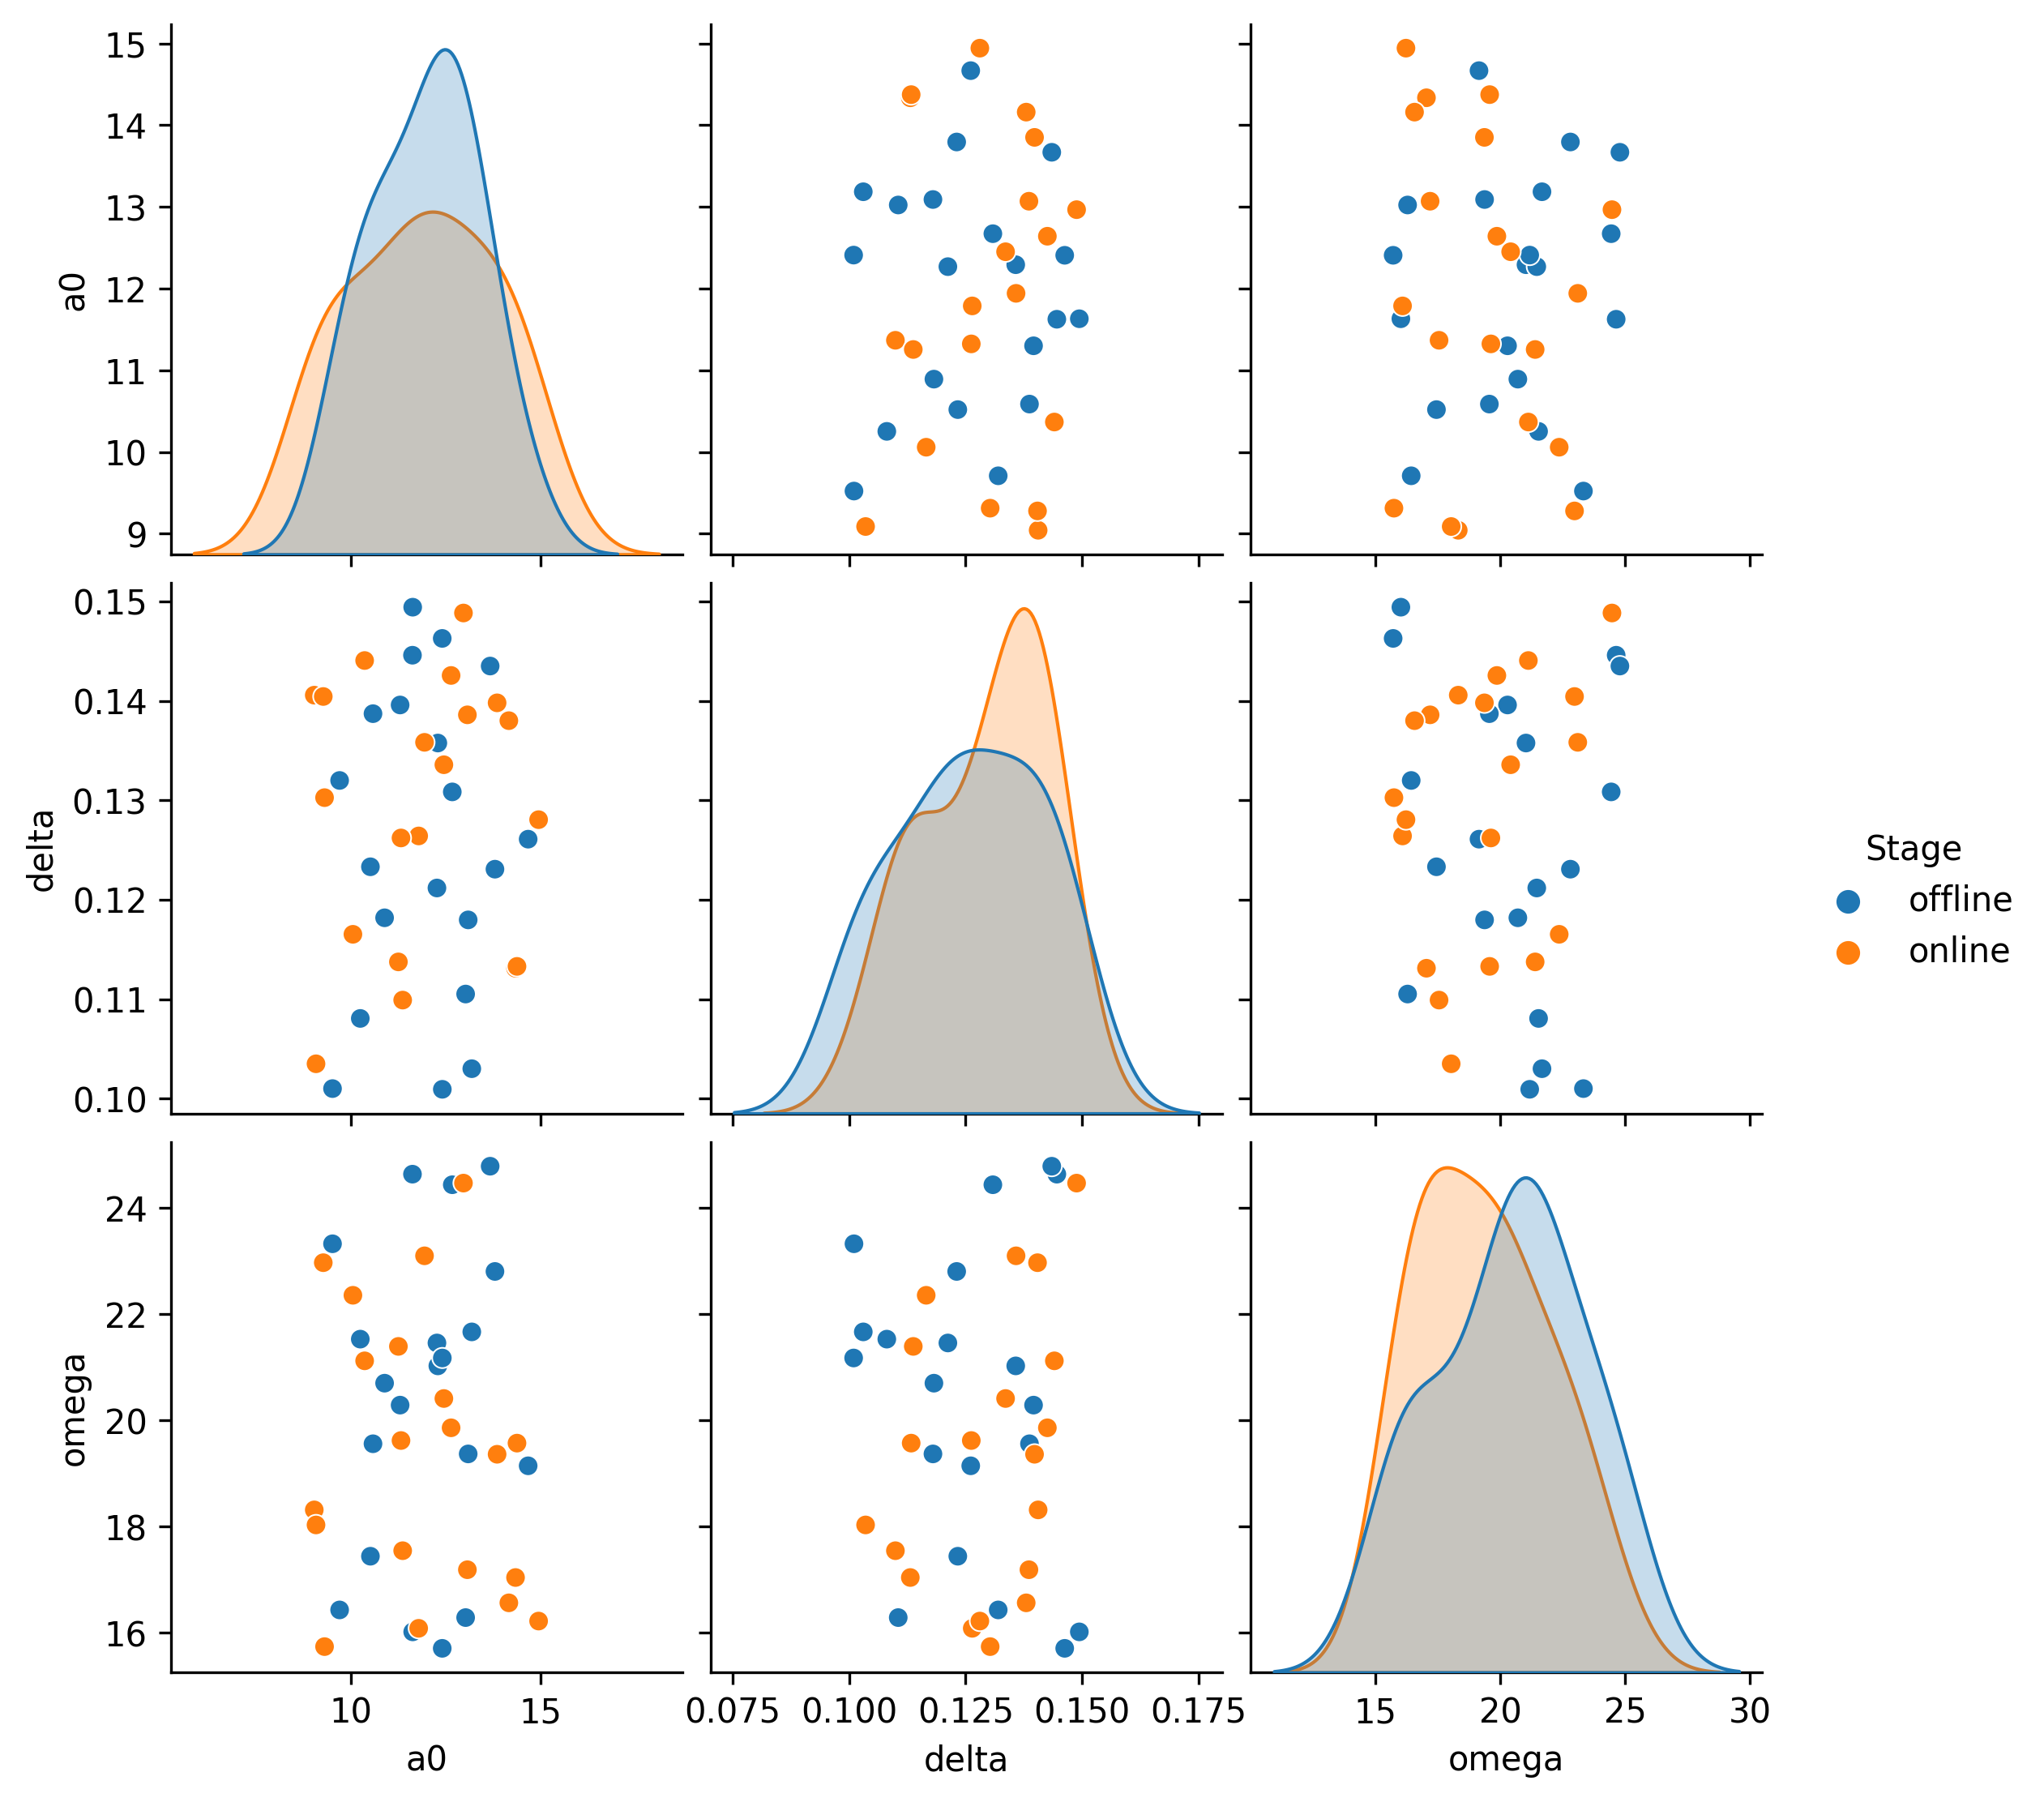
\includegraphics[width=\columnwidth]{research_project/piston/figures/hrom/mu_space.png}
%     \caption{Offline vs. Online parameter space for the Reduced Basis. 
%     20~parameters were selected for each stage.}
%     \label{fig:mu_space}
% \end{figure}

% \subsubsection{Benchmark}
% Figures \ref{fig:benchmark_validation} and \ref{fig:benchmark_online} for ROM errors.

% \begin{itemize}
%     \item The ROM achieves absolute accuracy ($10^{-6}$) for both validation and online sets.
% \end{itemize}

% \begin{figure}[!h]
%     \centering
%     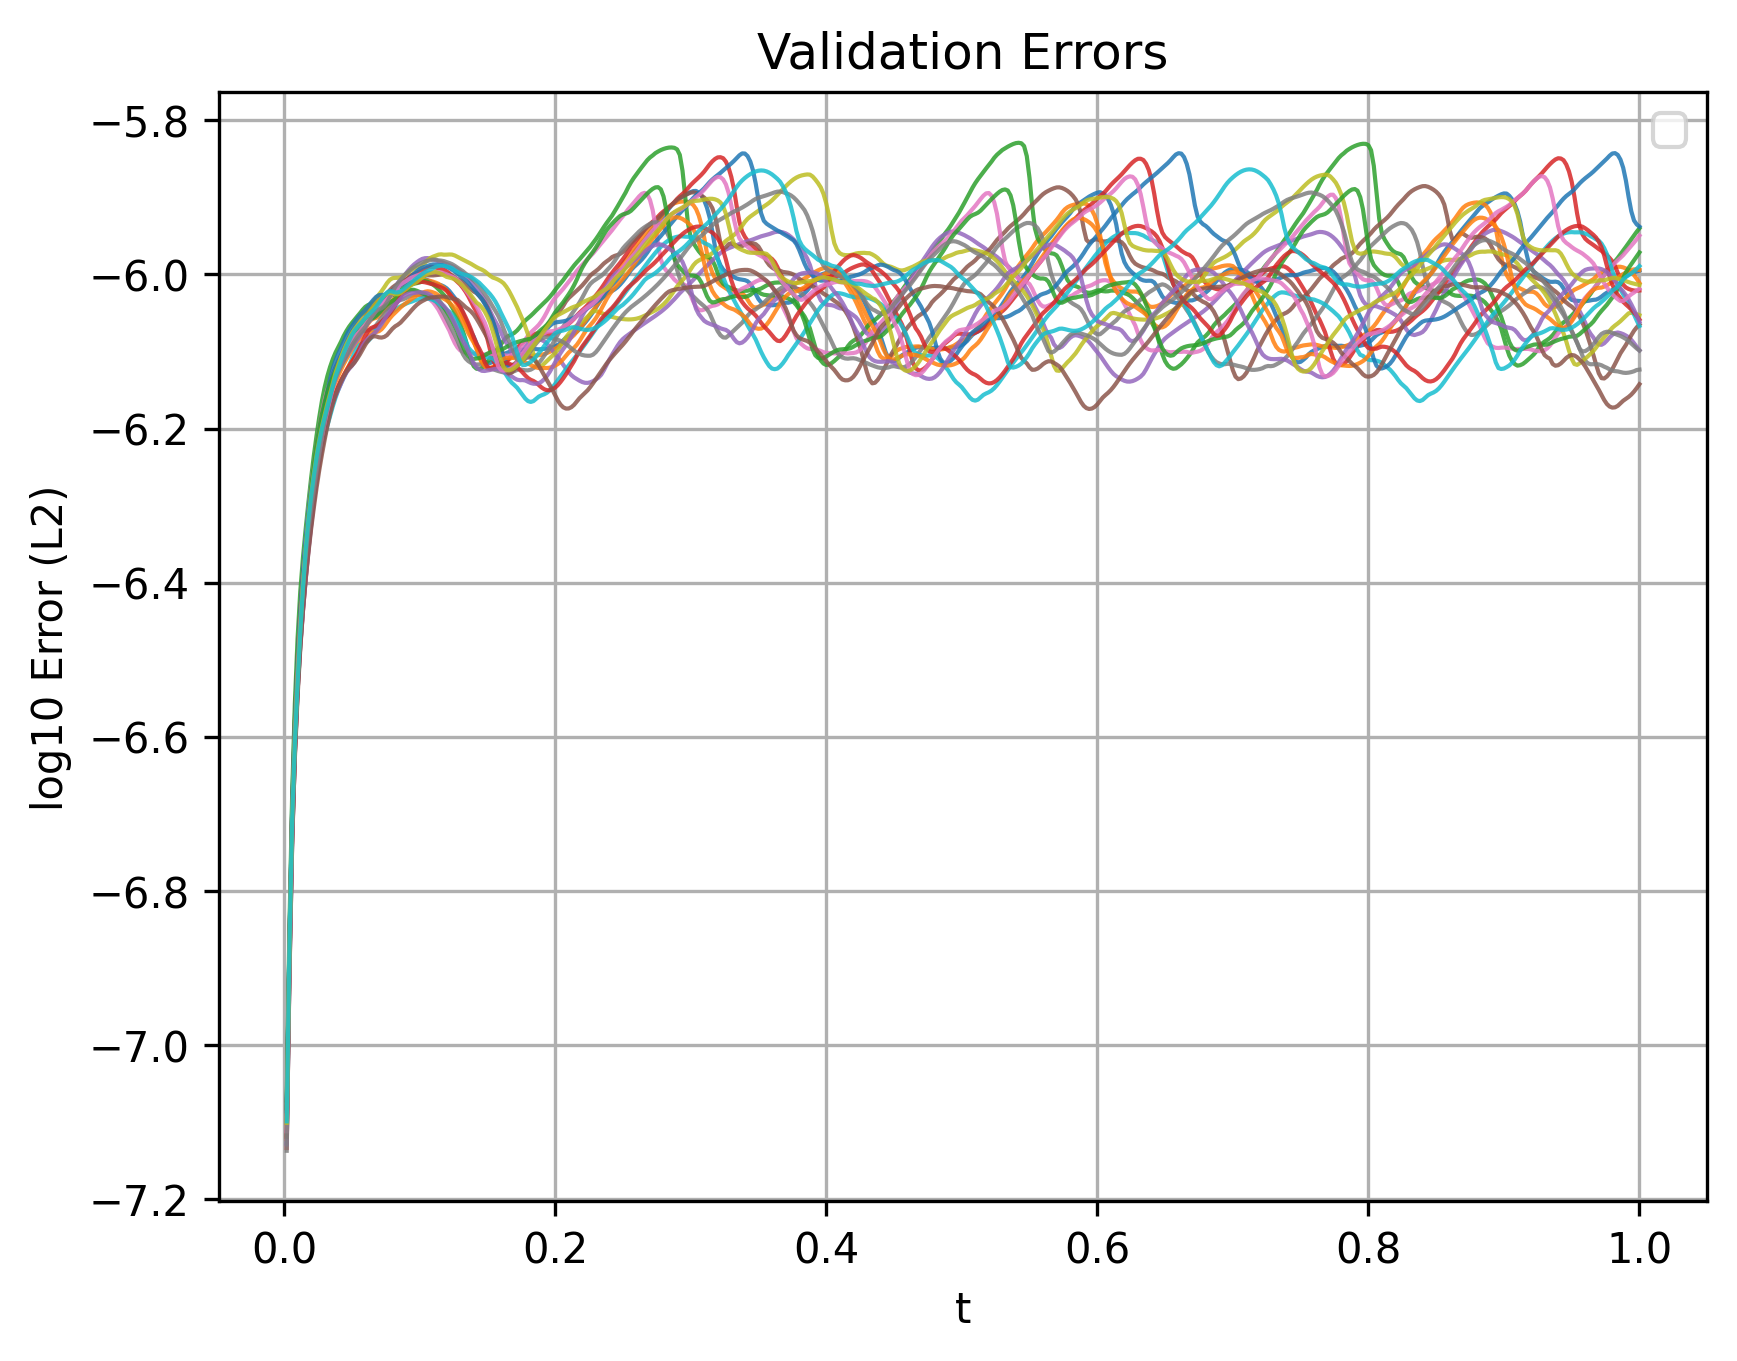
\includegraphics[width=\columnwidth]{research_project/piston/figures/hrom/benchmark/validation_errors.png}
%     \caption{(Benchmark) Validation errors.}
%     \label{fig:benchmark_validation}
% \end{figure}

% \begin{figure}[!h]
%     \centering
%     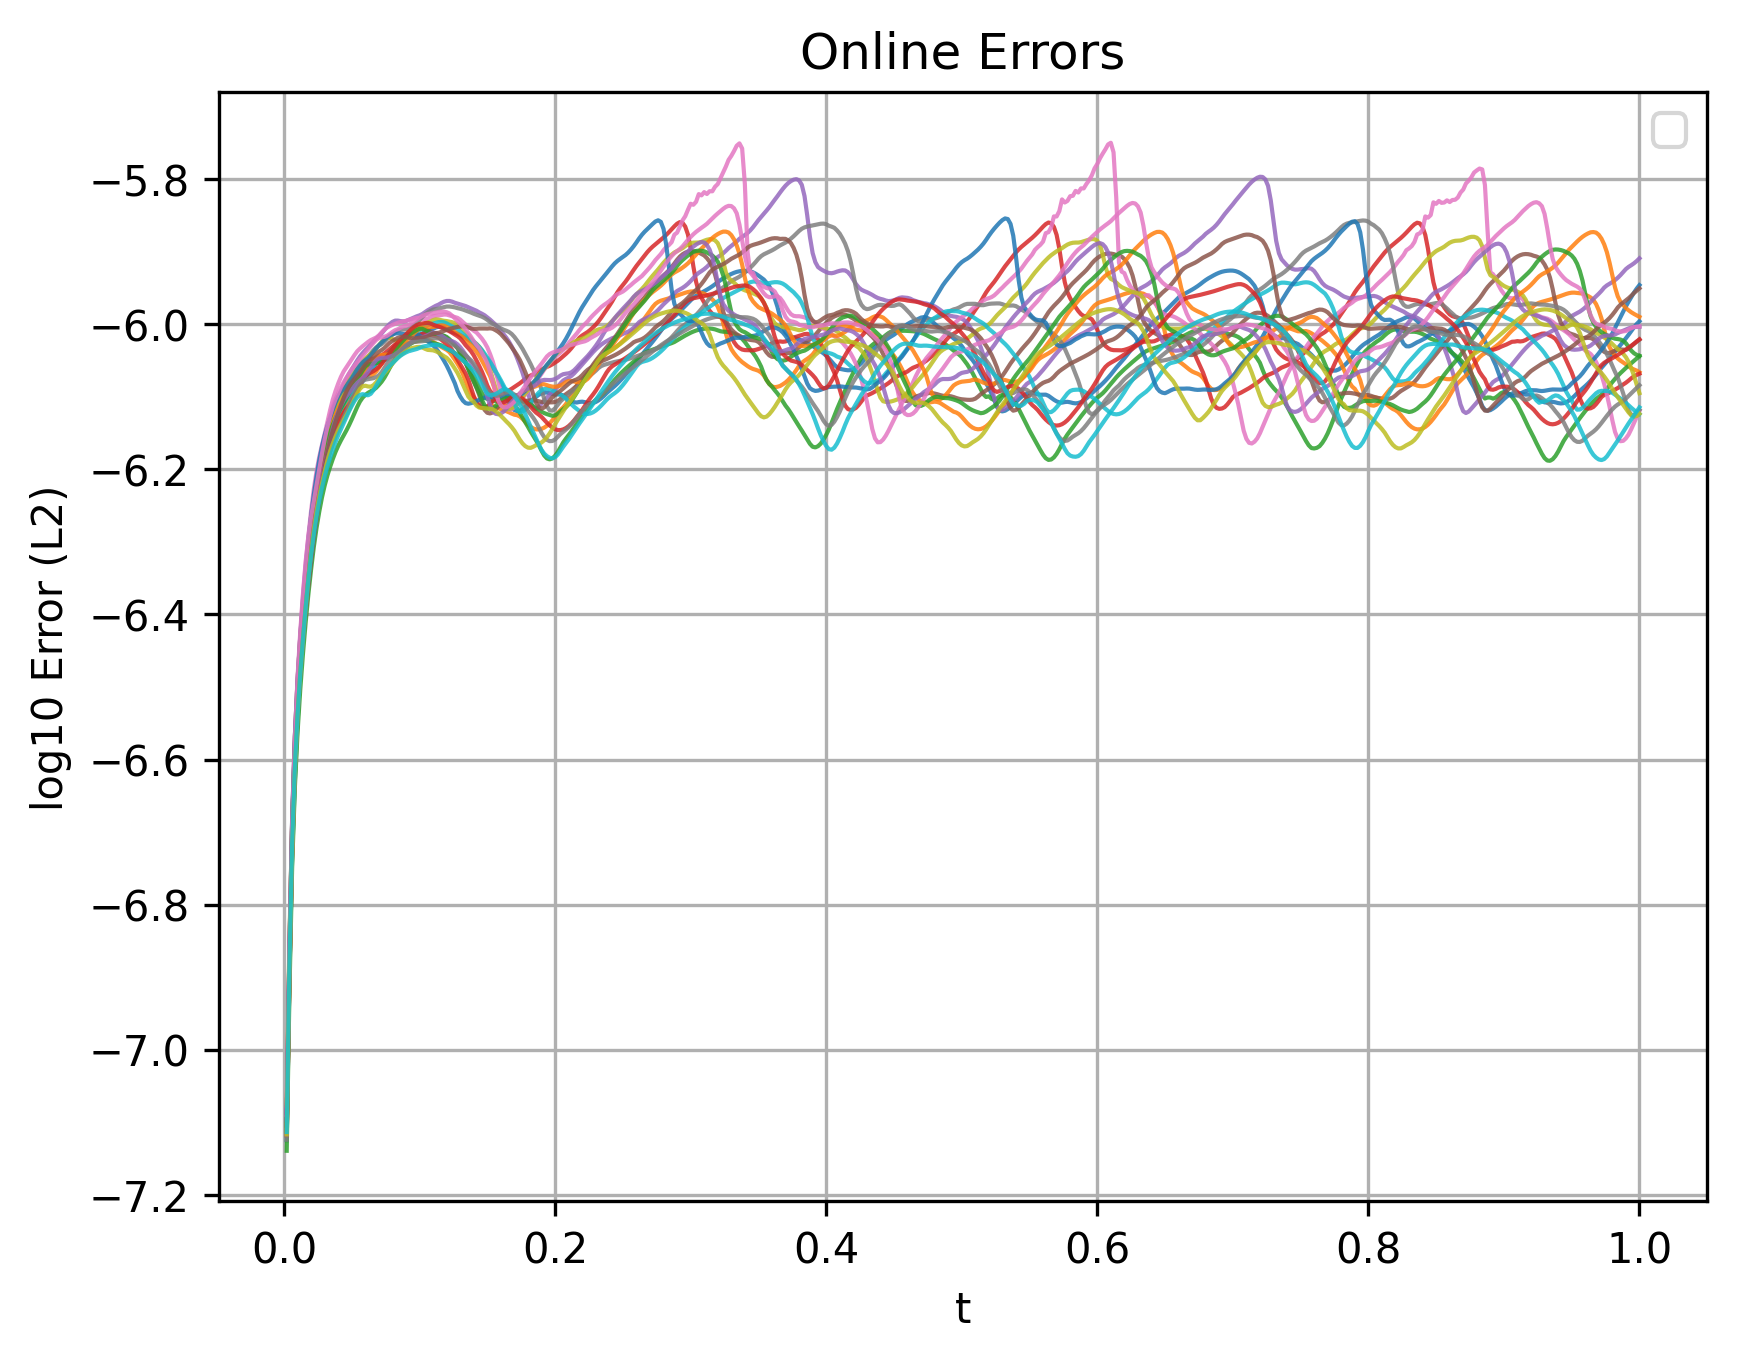
\includegraphics[width=\columnwidth]{research_project/piston/figures/hrom/benchmark/online_errors.png}
%     \caption{(Benchmark) Online errors.}
%     \label{fig:benchmark_online}
% \end{figure}

% \subsubsection{Half-Space}
% In Figure~\ref{fig:reduced_space} we plot the reduced space, with a clear non-linear character.

% Figures \ref{fig:halfspace_validation} and \ref{fig:halfspace_online} for ROM errors.


% \begin{itemize}
%     \item The ROM loses two orders of magnitude in accuracy ($10^{-4}$), and has the same behaviour for both the validation and online set.
% \end{itemize}

% \begin{figure}[!h]
%     \centering
%     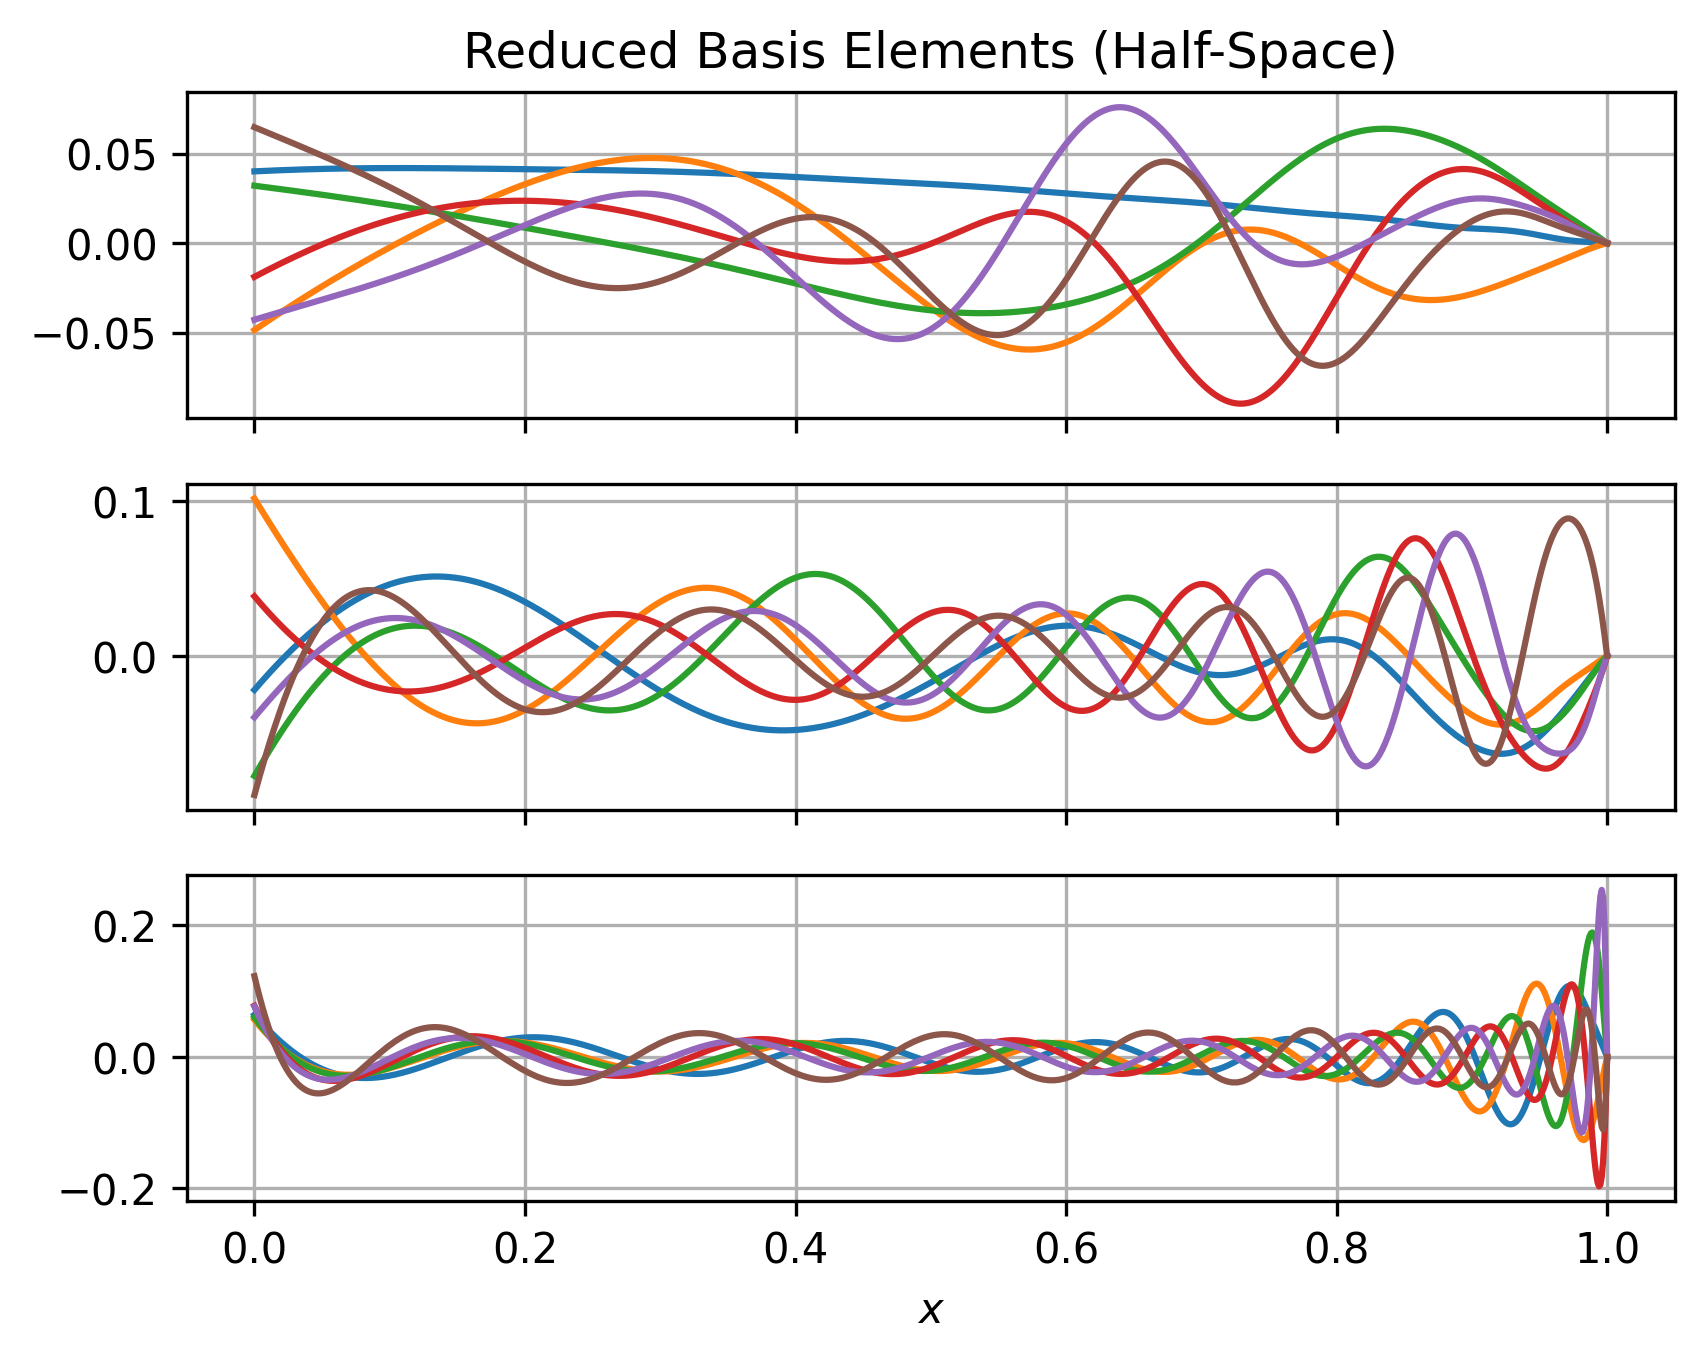
\includegraphics[width=\columnwidth]{research_project/piston/figures/hrom/reduced_basis.png}
%     \caption{(Half-Space) Reduced Space Elements. From top to bottom by decreasing level of energy. 
%     We can see how the first nodes have larger wavelengths, wereas the last ones present faster vibrations.}
%     \label{fig:reduced_space}
% \end{figure}

% \begin{figure}[!h]
%     \centering
%     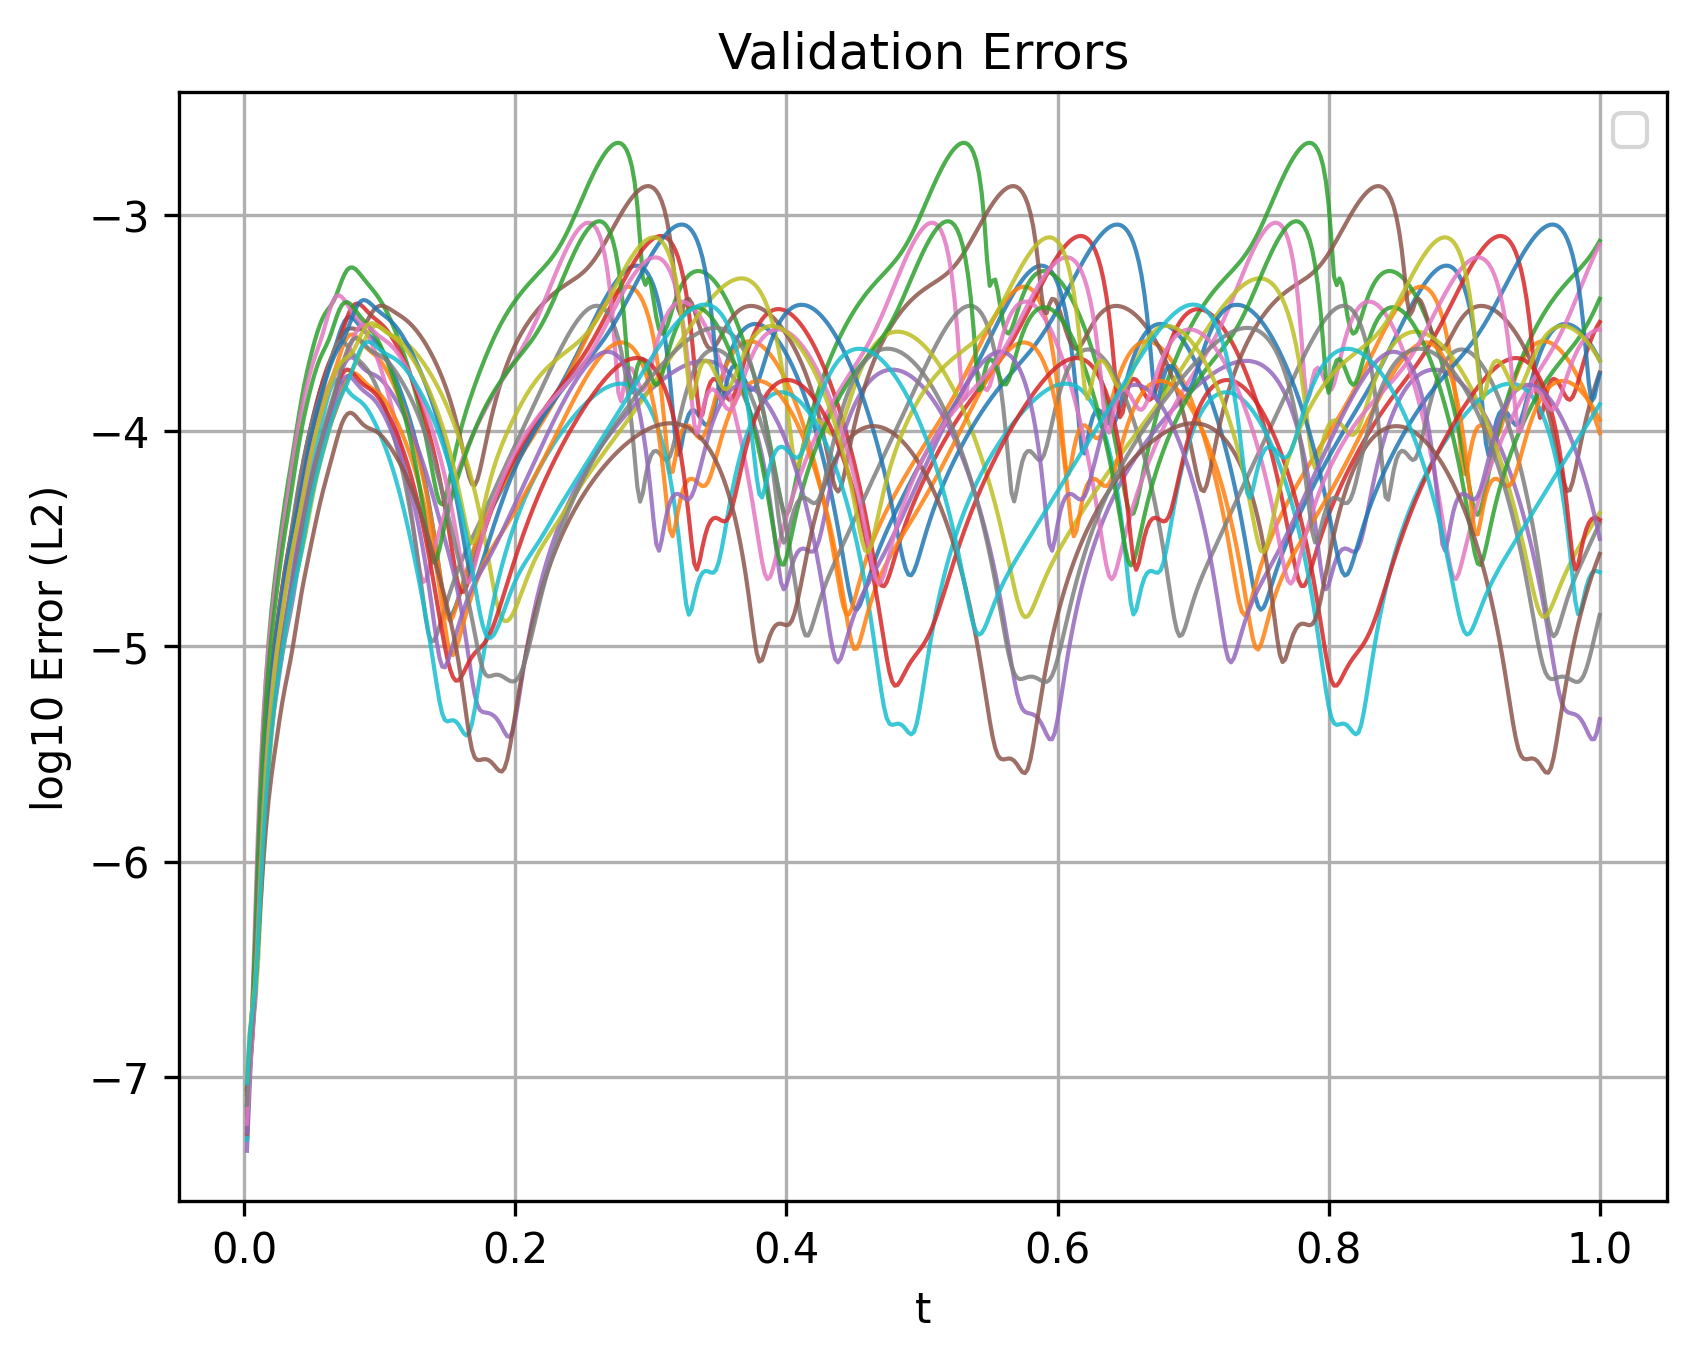
\includegraphics[width=\columnwidth]{research_project/piston/figures/hrom/half-space/validation_errors.png}
%     \caption{(Half-Space) Validation errors.}
%     \label{fig:halfspace_validation}
% \end{figure}

% \begin{figure}[!h]
%     \centering
%     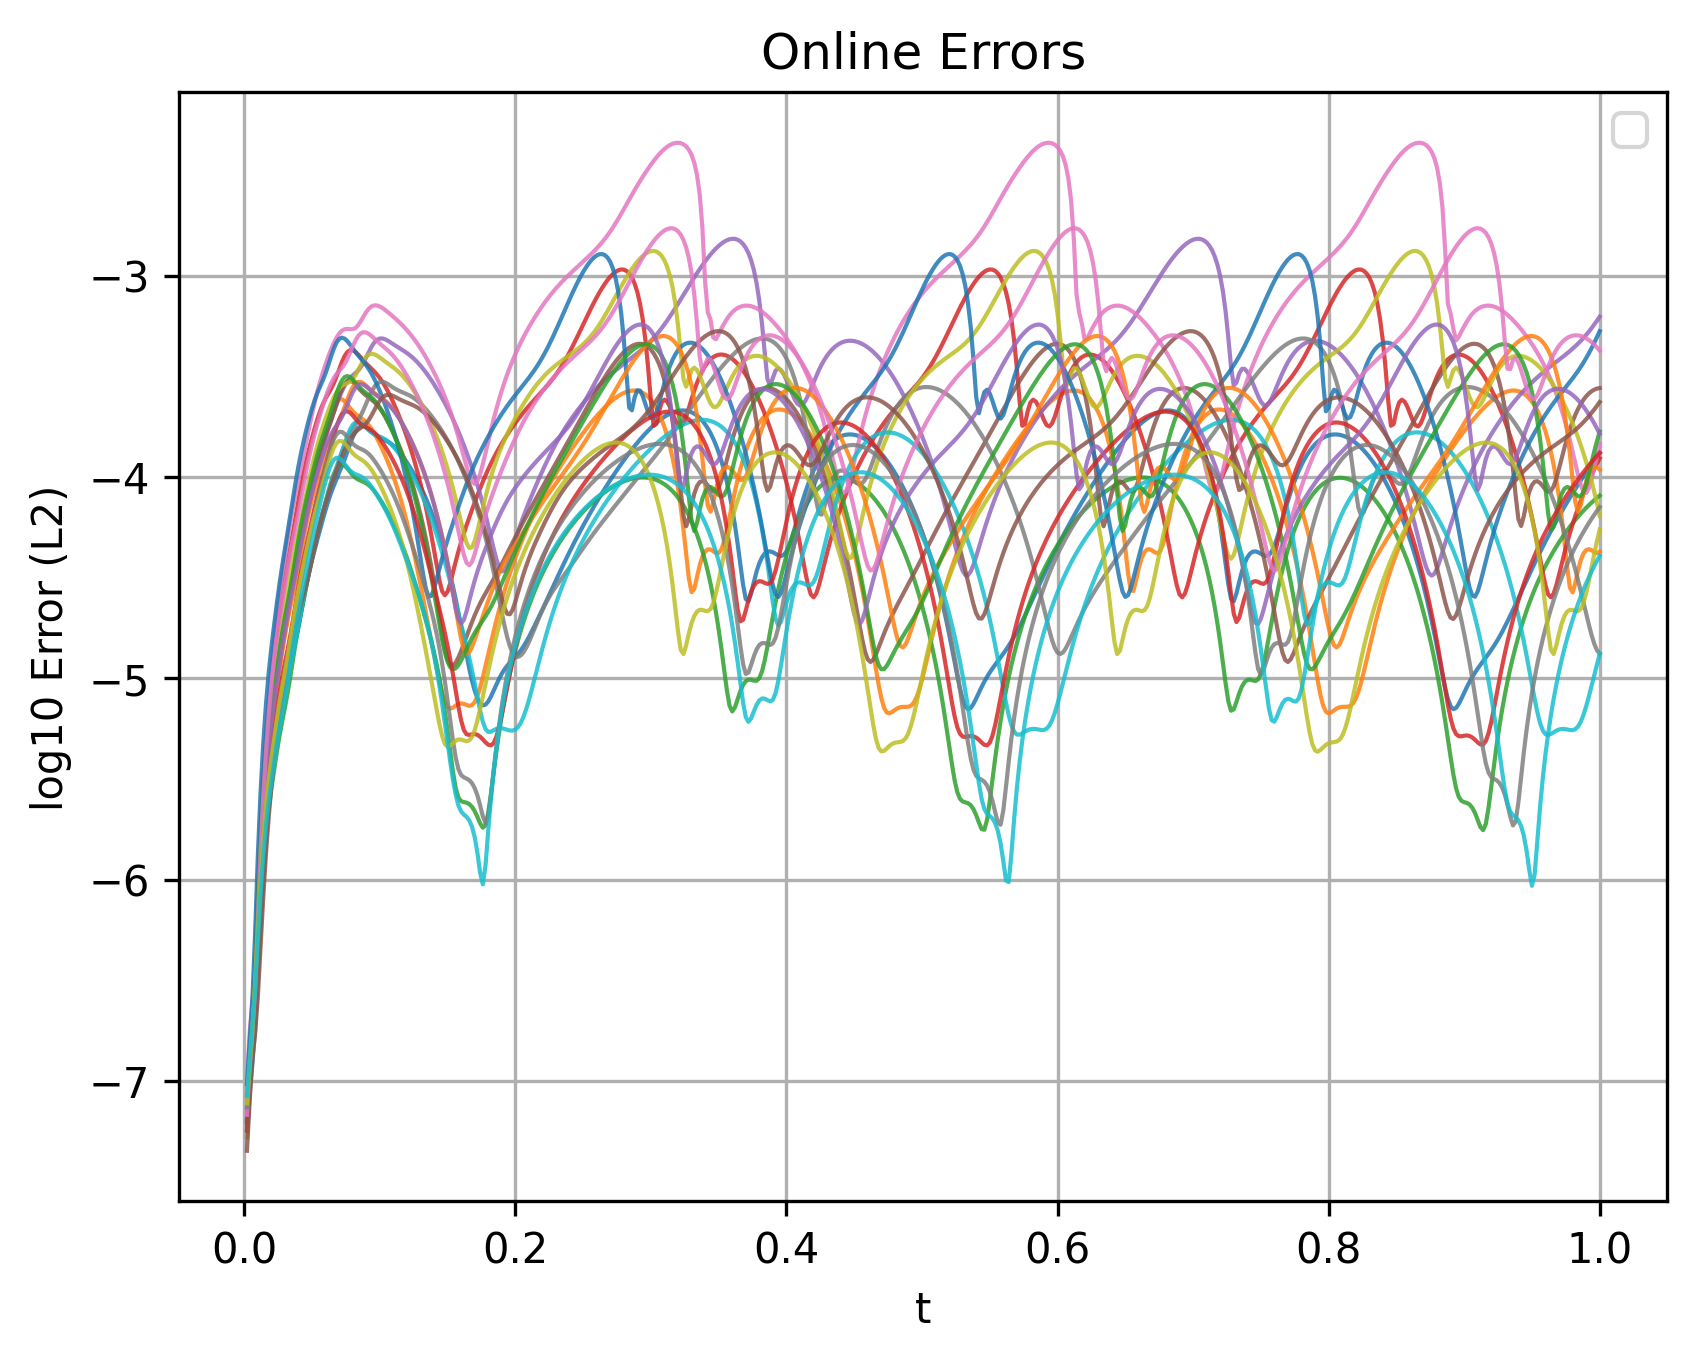
\includegraphics[width=\columnwidth]{research_project/piston/figures/hrom/half-space/online_errors.png}
%     \caption{(Half-Space) Online errors.}
%     \label{fig:halfspace_online}
% \end{figure}

% \subsubsection{Reduced Solution Space}
% Figures \ref{fig:reducedsolutionspace_validation} and \ref{fig:reducedsolutionspace_online} for ROM errors.

% \begin{itemize}
%     \item The ROM's accuracy is now widespread in terms of accuracy ($\left(10^{-6}, 10^{-4}\right)$), behaving slightly worse for the online set.
% \end{itemize}

% \begin{figure}[!h]
%     \centering
%     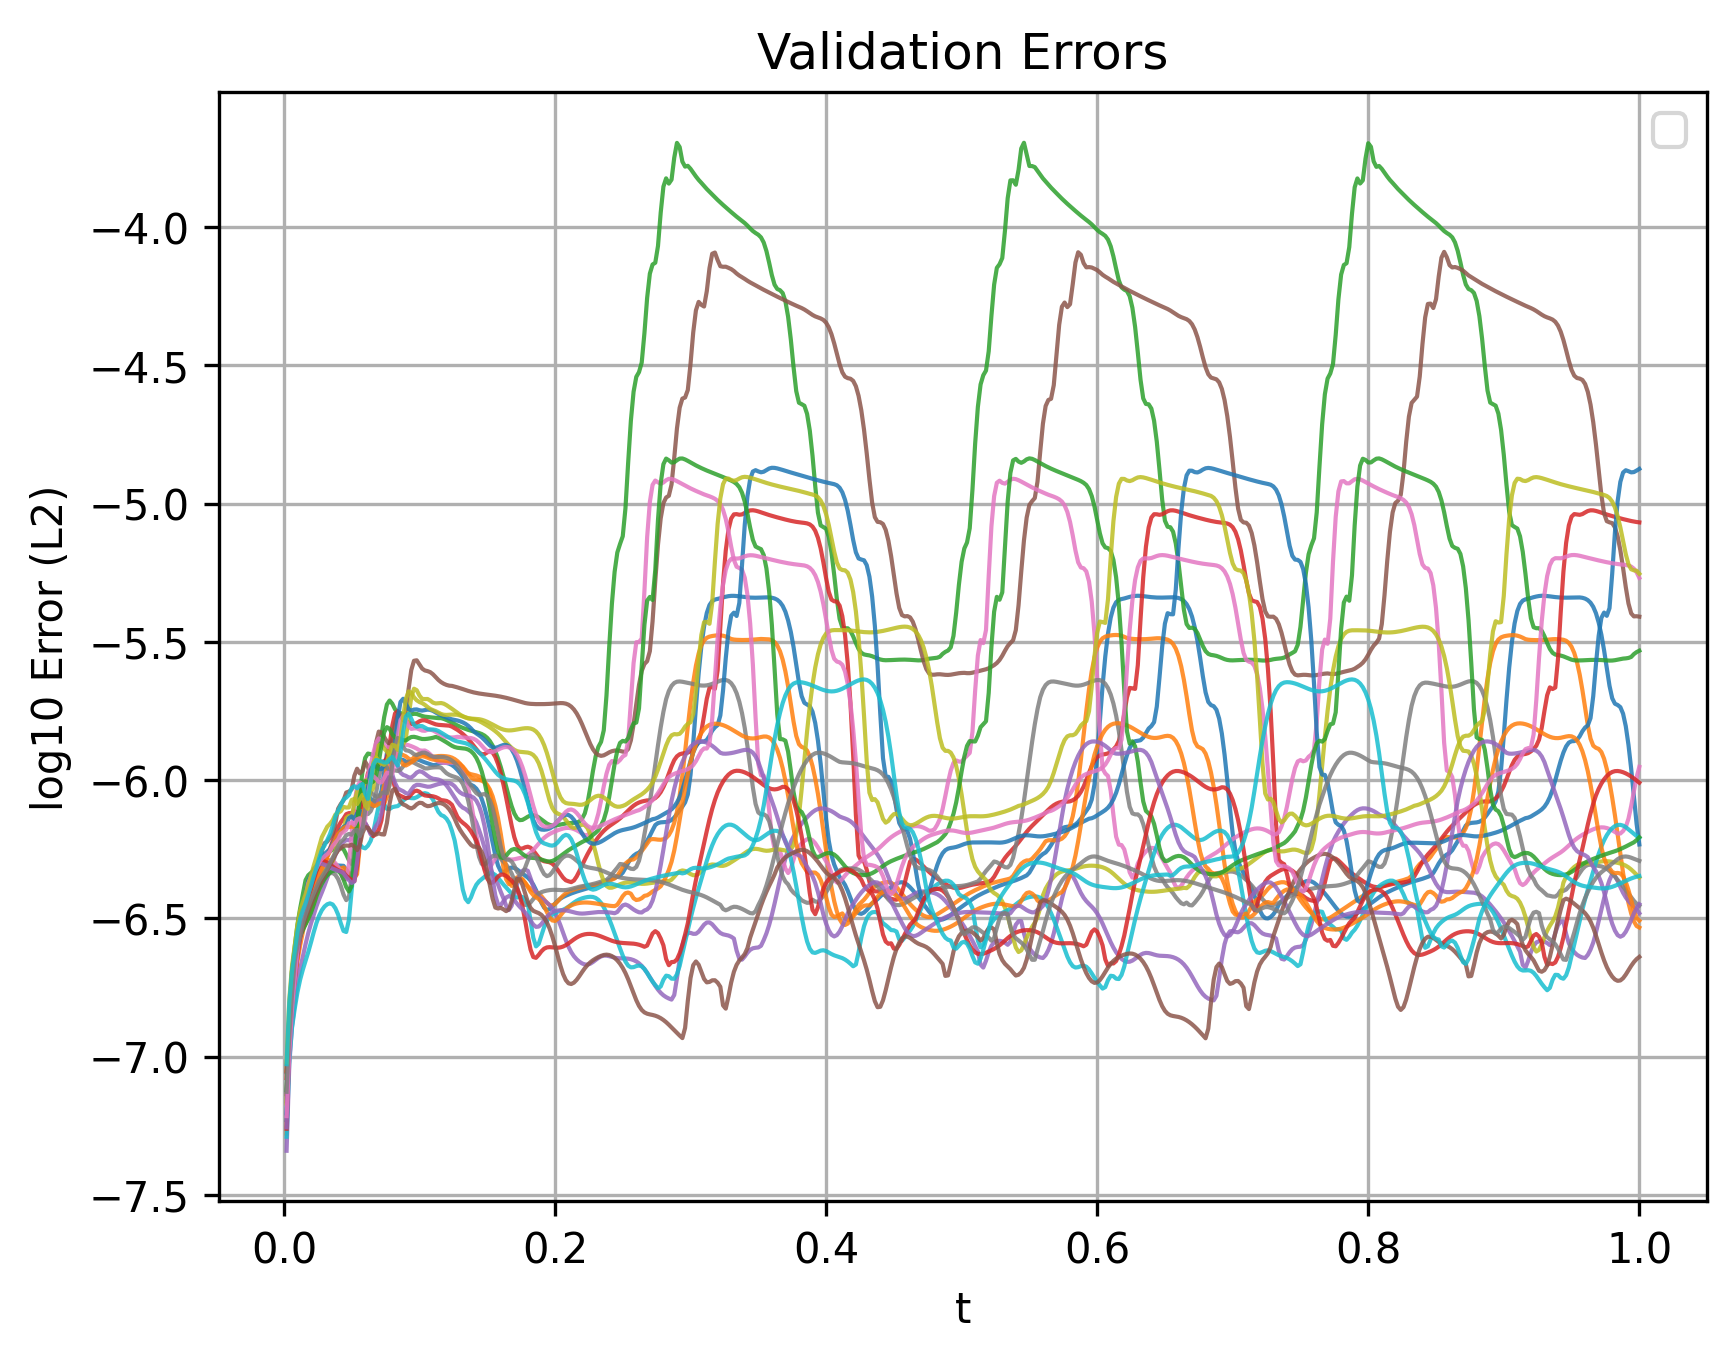
\includegraphics[width=\columnwidth]{research_project/piston/figures/hrom/reduced-solution-space/validation_errors.png}
%     \caption{(Reduced Solution Space) Validation errors.}
%     \label{fig:reducedsolutionspace_validation}
% \end{figure}

% \begin{figure}[!h]
%     \centering
%     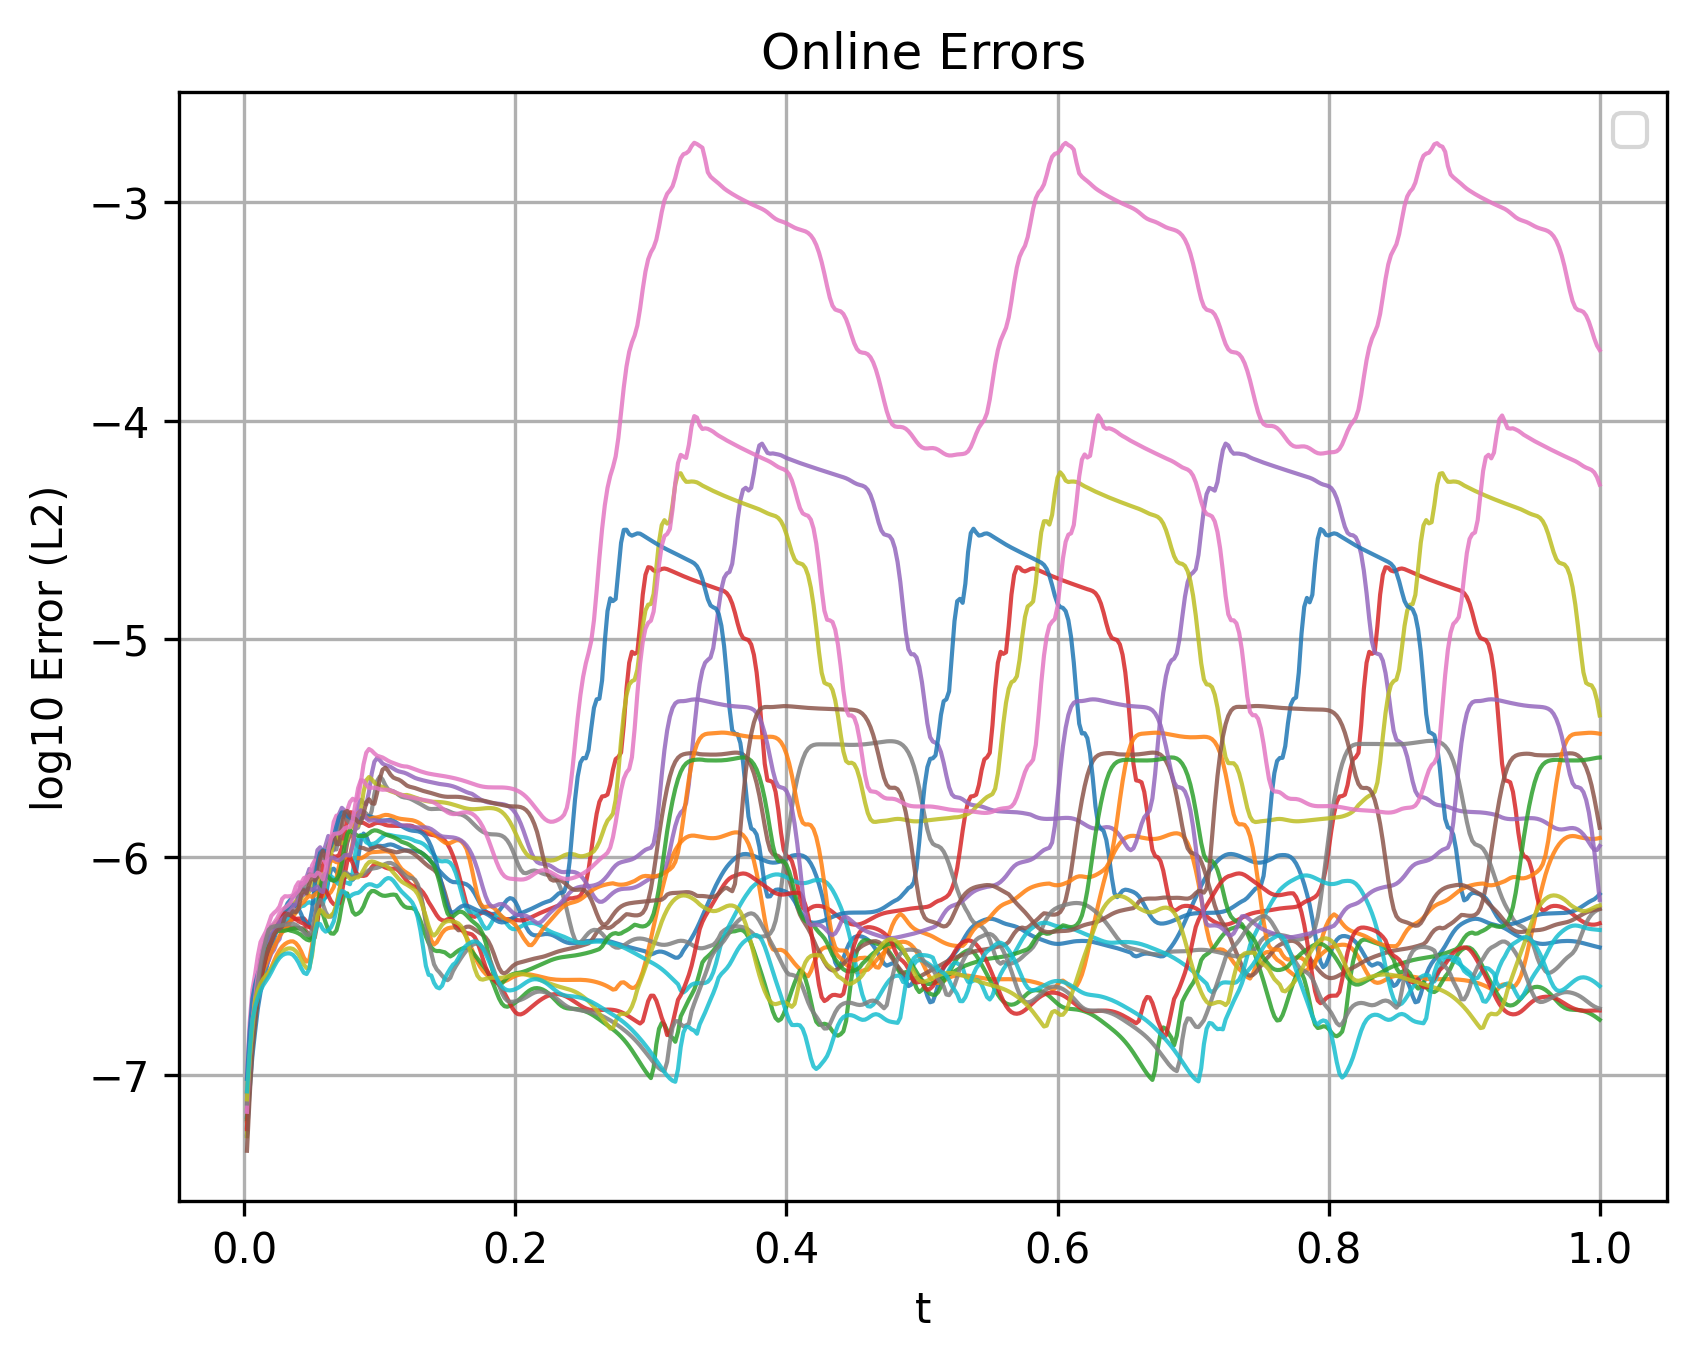
\includegraphics[width=\columnwidth]{research_project/piston/figures/hrom/reduced-solution-space/online_errors.png}
%     \caption{(Reduced Solution Space) Online errors.}
%     \label{fig:reducedsolutionspace_online}
% \end{figure}

% \newpage
% \subsection{Conclusions}
% Regarding discretization:
% \begin{itemize}
%     \item BDF-2 is a must (even higher order terms should be considered). 
%     It allows the reduction of timesteps to use, which speeds up the offline stage,
%     which is already quite heavy.
%     By introducing such scheme, for $t\in[0, 1.0]$, I could go from $Nt = 1000$ to $Nt = 500$, 
%     which reduced the offline to about an hour instead of two/three hours.
% \end{itemize}

% Regarding model reduction:
% \begin{itemize}
%     \item The model captures correctly nonlinearities.
%     \item Linear operators are so simple a few collateral basis elements are enough to reduce them. 
%     This is due to the simplicity of the jacobian transformation between moving and reference domains.
%     \begin{itemize}
%         \item No point in playing with the tolerances for linear operators.
%     \end{itemize}
%     \item Reduction of the nonlinear term is a costly operation, because the integral of the basis elements cannot be efficiently computed due to its global support.
%     \item If collateral basis elements for the nonlinear operator are neglected, the solution loses its physical accuracy.
%     \item The reduced basis can be trimed without affecting too much the solution (not as much as the nonlinear operator).
%     \item It would be interesting to have analytical results about the relation between parameter space tolarence and online errors.
% \end{itemize}

% \subsection{Future Work}
% With this work so far we have proved that the ROM with reduced basis for the solution \textit{and} the operators in moving domains works.

% There is one flaw though, we can only assess the bondness of the ROM by computing the FOM solution too for the same parametrization.
% This makes it cumbersome, since we would like to compute the error without having to compute the FOM solution too.

% There are two possible paths now:
% \begin{itemize}
%     \item Extend the same procedure to a 2D domain.
%     \item Certify the ROM with the development of \textit{a posteriori} error computations.
% \end{itemize}

% Calculation for a 2D domain is more number-crunching and coding work, no new knowledge will be learned.
% Bug prone, non-mathematical work overhead (implementation details).
% If achieved, none of the models are certified: online errors can only be computed by solving the FOM problem too.
% Adds to the body of knowledge in a can-be-done way, not learning anything we cannot learn from the 1D problem
% about the implementation details. 

% Calculation of a posteriori error computation requires error bounds and the extension of some offline structures.
% More uncertainty is involved, but it gives actual closure to the ROM problem.
% Mathematical work, adds to the body of knowledge.

% \subsubsection{Extension to 2D}
% Extension of the procedure to a 2D setting would require:
% \begin{itemize}
%     \item Construction of a FOM solver. Requirements:
%     \begin{itemize}
%         \item To build the final algebraic operator by the sum of diverse operators.
%         \item To be semi-implicit. 
%     \end{itemize}
%     \item Rewriting the (M)DEIM reductors, they assume a 1D setting.
%     \item Module to create harmonic extensions for lifting and mesh displacement.
%     \item Updating the move mesh module. Right now it simply scales the mesh.
%     \item Learning to use Paraview to plot the solution.
% \end{itemize}

% \subsubsection{ROM Certification: A Posteriori Errors}
% There is previous work on time-dependent matrices for fixed domains.

% A posteriori errors would require:
% \begin{itemize}
%     \item Construction of Rietz reprensentant.
%     \item Calculation of eigenvalues.
%     \item Literature reading.
% \end{itemize}

\end{document}